% ULaTeX2e, calling the article.cls class and 12-point type.

\documentclass[12pt]{article}

% My packages

\usepackage{framed, color}
\usepackage{soul}
\definecolor{blu}{rgb}{0,0,1}
\newcommand{\td}[1]{{\color{blu}\hl{TODO: #1}}}
\usepackage{graphicx}
\usepackage{amsthm}
\newtheorem{mydef}{Definition}
\usepackage{dcolumn}
\usepackage{multirow}
\usepackage{booktabs}
\newcolumntype{d}{D{.}{.}{4.0}}
\newcolumntype{s}{D{.}{.}{1.4}}

% Users of the {thebibliography} environment or BibTeX should use the
% scicite.sty package, downloadable from *Science* at
% www.sciencemag.org/about/authors/prep/TeX_help/ .
% This package should properly format in-text
% reference calls and reference-list numbers.

\usepackage{scicite}

% Use times if you have the font installed; otherwise, comment out the
% following line.

\usepackage{times}

% The preamble here sets up a lot of new/revised commands and
% environments.  It's annoying, but please do *not* try to strip these
% out into a separate .sty file (which could lead to the loss of some
% information when we convert the file to other formats).  Instead, keep
% them in the preamble of your main LaTeX source file.


% The following parameters seem to provide a reasonable page setup.

\topmargin 0.0cm
\oddsidemargin 0.2cm
\textwidth 16cm 
\textheight 21cm
\footskip 1.0cm


%The next command sets up an environment for the abstract to your paper.

\newenvironment{sciabstract}{%
\begin{quote} \bf}
{\end{quote}}


% If your reference list includes text notes as well as references,
% include the following line; otherwise, comment it out.

\renewcommand\refname{References and Notes}

% The following lines set up an environment for the last note in the
% reference list, which commonly includes acknowledgments of funding,
% help, etc.  It's intended for users of BibTeX or the {thebibliography}
% environment.  Users who are hand-coding their references at the end
% using a list environment such as {enumerate} can simply add another
% item at the end, and it will be numbered automatically.

\newcounter{lastnote}
\newenvironment{scilastnote}{%
\setcounter{lastnote}{\value{enumiv}}%
\addtocounter{lastnote}{+1}%
\begin{list}%
{\arabic{lastnote}.}
{\setlength{\leftmargin}{.22in}}
{\setlength{\labelsep}{.5em}}}
{\end{list}}


% Include your paper's title here

\title{Hysteresis in human computation:\\ how one task affects another} 


% Place the author information here.  Please hand-code the contact
% information and notecalls; do *not* use \footnote commands.  Let the
% author contact information appear immediately below the author names
% as shown.  We would also prefer that you don't change the type-size
% settings shown here.

\author
{Edward Newell \\ Derek Ruths\\
\\
\normalsize{\texttt{edward.newell@mail.mcgill.ca}}\\
\normalsize{\texttt{druths@networkdynamics.org}}\\
\normalsize{School of computer science, McGill University,}\\
\normalsize{3630 rue University, Montreal, Quebec, H3A 0C6, Canada}\\
\\
}

% Include the date command, but leave its argument blank.

\date{}



%%%%%%%%%%%%%%%%% END OF PREAMBLE %%%%%%%%%%%%%%%%



\begin{document} 

% Double-space the manuscript.

\baselineskip24pt

% Make the title.

\maketitle 



% Place your abstract within the special {sciabstract} environment.

\begin{sciabstract}

Faced with the ever-growing scale and complexity of data, researchers and
industry are increasingly relying on \textit{human computation} as a means
to extract useful knowledge.  Microtask
platforms, like Amazon Mechanical Turk, act like a human compute server,
making it possible to access human cognition quickly and inexpensively. 
This has lead to broad adoption across a spectrum of disciplines
in the social sciences and computer science, as well as in research into 
medical imaging technologies and other applications where expert opinion 
would normally be sought.  Here we show that an inherent
feature of microtask platforms and most crowdsourcing settings---the 
repetition of similar tasks---acts as a strong, but as yet unexplored source 
of bias.  These \textit{intertask effects} rival the
severity of overtly framing a task's purpose.  
Using image-labeling as a canonical microtask, we show that prior 
tasks influence the content that workers focus on, and the richness and
specialization of their vocabulary.    
While intertask effects can be a source of systematic bias, our
results suggest that, when properly controlled, they might be leveraged
to hone worker focus and specificity, and could play a key role in designing 
tasks that elicit expert-level judgments.
\end{sciabstract}

\section*{Main text}
Microtask platforms are online marketplaces in which \textit{requesters} 
post batches of tasks, and \textit{workers} complete them
for remuneration, a sense of purpose, and for fun
\cite{kazai2013analysis,Antin20122925}.  
Typical tasks include tagging and categorizing images 
\cite{6116320,Zhai2012357}, transcribing voice recordings 
\cite{chandler2013breaking,paolacci2010running}
or handwritten notes \cite{Berinsky2012351,Finnerty2013}, and judging the 
relevancy of search results 
\cite{le2010ensuring,grady2010crowdsourcing,alonso2009can,kazai2013analysis}.

While microtask platforms have been widely adopted as a research tool,
computer scientists also hold such platforms as the object of 
research, viewing  microtask platforms as a new kind of computing 
architecture.  In analogy to CPUs (central 
processing units) and GPUs (graphics processing units), 
Davis \textit{et al} invoked the \textit{human processing unit}, or HPU \cite{5543192}.
Meanwhile, researchers have sought to define a basic HPU instruction set, and
libraries for HPU programming are under active development
 \cite{little2010turkit,minder2011crowdlang,minder2012crowdlang,kittur2011crowdforge}.  

Given the increasing prevalence of microtask-based research methods, there
is a desire to understand the factors affecting the reliability of HPU
outputs.  Researchers have investigated task-design parameters such as the 
level of pay \cite{kazai2013analysis}, the training \cite{le2010ensuring} and 
pre-screening \cite{paolacci2010running} of workers, and user-interface 
design factors \cite{Finnerty2013}.  
Researchers have also investigated \textit{framing} effects, 
such as the effects of describing the workflow context 
\cite{Kinnaird2012281}, the purpose of tasks 
\cite{chandler2013breaking}, or altering the problem description
\cite{thibodeau2013natural}.  Results in psychology show that people are 
susceptible to various kinds of priming 
\cite{BJOP1796,No2007,beller1971priming}, and, in particular, 
task-repetition effects \cite{Gass1999549,sohn2001task}.  
Yet to our knowledge, no study has investigated the practical ramifications 
of intertask effects on human computation. The experiments we 
present here show that, unlike CPUs and GPUs, HPUs are subject to 
\textit{hysteresis}, meaning that their outputs depend on the 
\textit{history} of their inputs.  

We investigated intertask effects using image-labeling tasks on the Amazon 
Mechanical Turk (MTurk) microtask platform.  Image-labeling tasks are among
the most common MTurk tasks \cite{chandler2013breaking,Berinsky2012351,Finnerty2013,paolacci2010running}.  This trend will probably continue 
in the long term because of their role in computer vision research 
\td{find another application} \cite{5543192}.  In microtask platforms, it is typical for work to be divided 
into bundles; on MTurk, these bundles are called Human Intelligence Tasks 
(HITs). Because of this bundling pattern, even if workers perform only one 
HIT, the opportunity for intertask effects arises.  For clarity, 
we will use ``task'' to mean the smallest repeatable unit of work, which, 
in our study, consists of labeling a single image.

In our first experiment, which we will refer to as 
\textit{intertask-food-objects}, workers were either assigned to the 
\textit{food} or \textit{objects} treatment.  Workers in these treatments
performed a set of five \textit{initial tasks}, which involved labeling
images depicting either food or (non-food) objects, depending on the worker's 
treatment (see Fig.~\ref{fig:task}A and B).  Following the initial 
tasks, workers performed five \textit{test tasks}, which were identical for 
both treatments.  The test tasks contained images depicting a 
mixture of food and other objects (see Fig.~\ref{fig:task}C).  Five initial 
tasks, together with the test tasks, comprised one HIT 
(\# workers were only allowed to participate once). During the HIT, workers 
were presented images one at a time, and, crucially, there was no distinction
or interruption between the initial and test tasks.

A $\chi^2$ test (\#) shows that the frequency of word usage by
workers in the \textit{food} and \textit{objects} treatments differed
significantly during test tasks, even though the test tasks were identical 
for the treatments.  This shows that earlier tasks have a 
significant effect on later ones, and raises concerns about the 
design of microtasks, and possibly the microtask methodology itself.

While this affirms the \textit{existence} of intertask effects, we wish to
understand the nature and severity of the bias induced by prior task 
exposure.  To formalize a notion of the extent of bias, we must first 
acknowledge that workers' responses to microtasks
carry an element of stochasticity: two workers will not, in general, provide
the same response to a given task.  Because worker responses are stochastic,
we take the extent of bias, $\theta$, to be the total shift in probability 
mass, for giving certain responses (i.e. certain words),
caused by a perturbation like intertask effects (\# in other words, the 
bias is the L1-distance between the probability distributions for responses
under one treatment, to that for responses under another.)

It is difficult to measure the change in a probability distribution based on
samples alone (\#), so we reformulate the problem slightly. Consider that,  
no matter the ultimate purpose of a microtask study, a microtask response
is used in \textit{some kind} of subsequent decision or 
further processing.
We denote this dowstream decision by $\mathcal{D}$.  Since $\mathcal{D}$
takes a microtask response as input, biases in the microtask response will 
in general lead to biases in the output of $\mathcal{D}$.  
We can make use of this fact, 
by placing a machine learning algorithm (a classifier), in the role of 
$\mathcal{D}$.  This classifier takes as input a worker's responses to test 
tasks, from which it learns to infer the worker's treatment 
(i.e. the initial tasks she was given). 
Intuitively, the classifier's ability to infer the worker's treatment
depends on how strongly the exposure to prior tasks influences responses to 
subsequent ones.  Formally, the bias, $\theta$, is bounded 
by the accuracy of the classifier, $\eta$ (\#):
\begin{equation}
	\theta \geq 2\eta - 1.
	\label{l1}
\end{equation}
Thus, measuring the performance of the classifier allows us to establish a
lower bound on the extent of bias. This approach can be used to bound the 
bias induced by any purturbation, including both intertask effects and 
framing.  Bias ranges from 0 (meaning there are no intertask effects), to 1 
(or 100\%) (meaning that changing initial tasks leads to a completely 
different set of responses to test tasks).

\begin{figure}
	\centering
	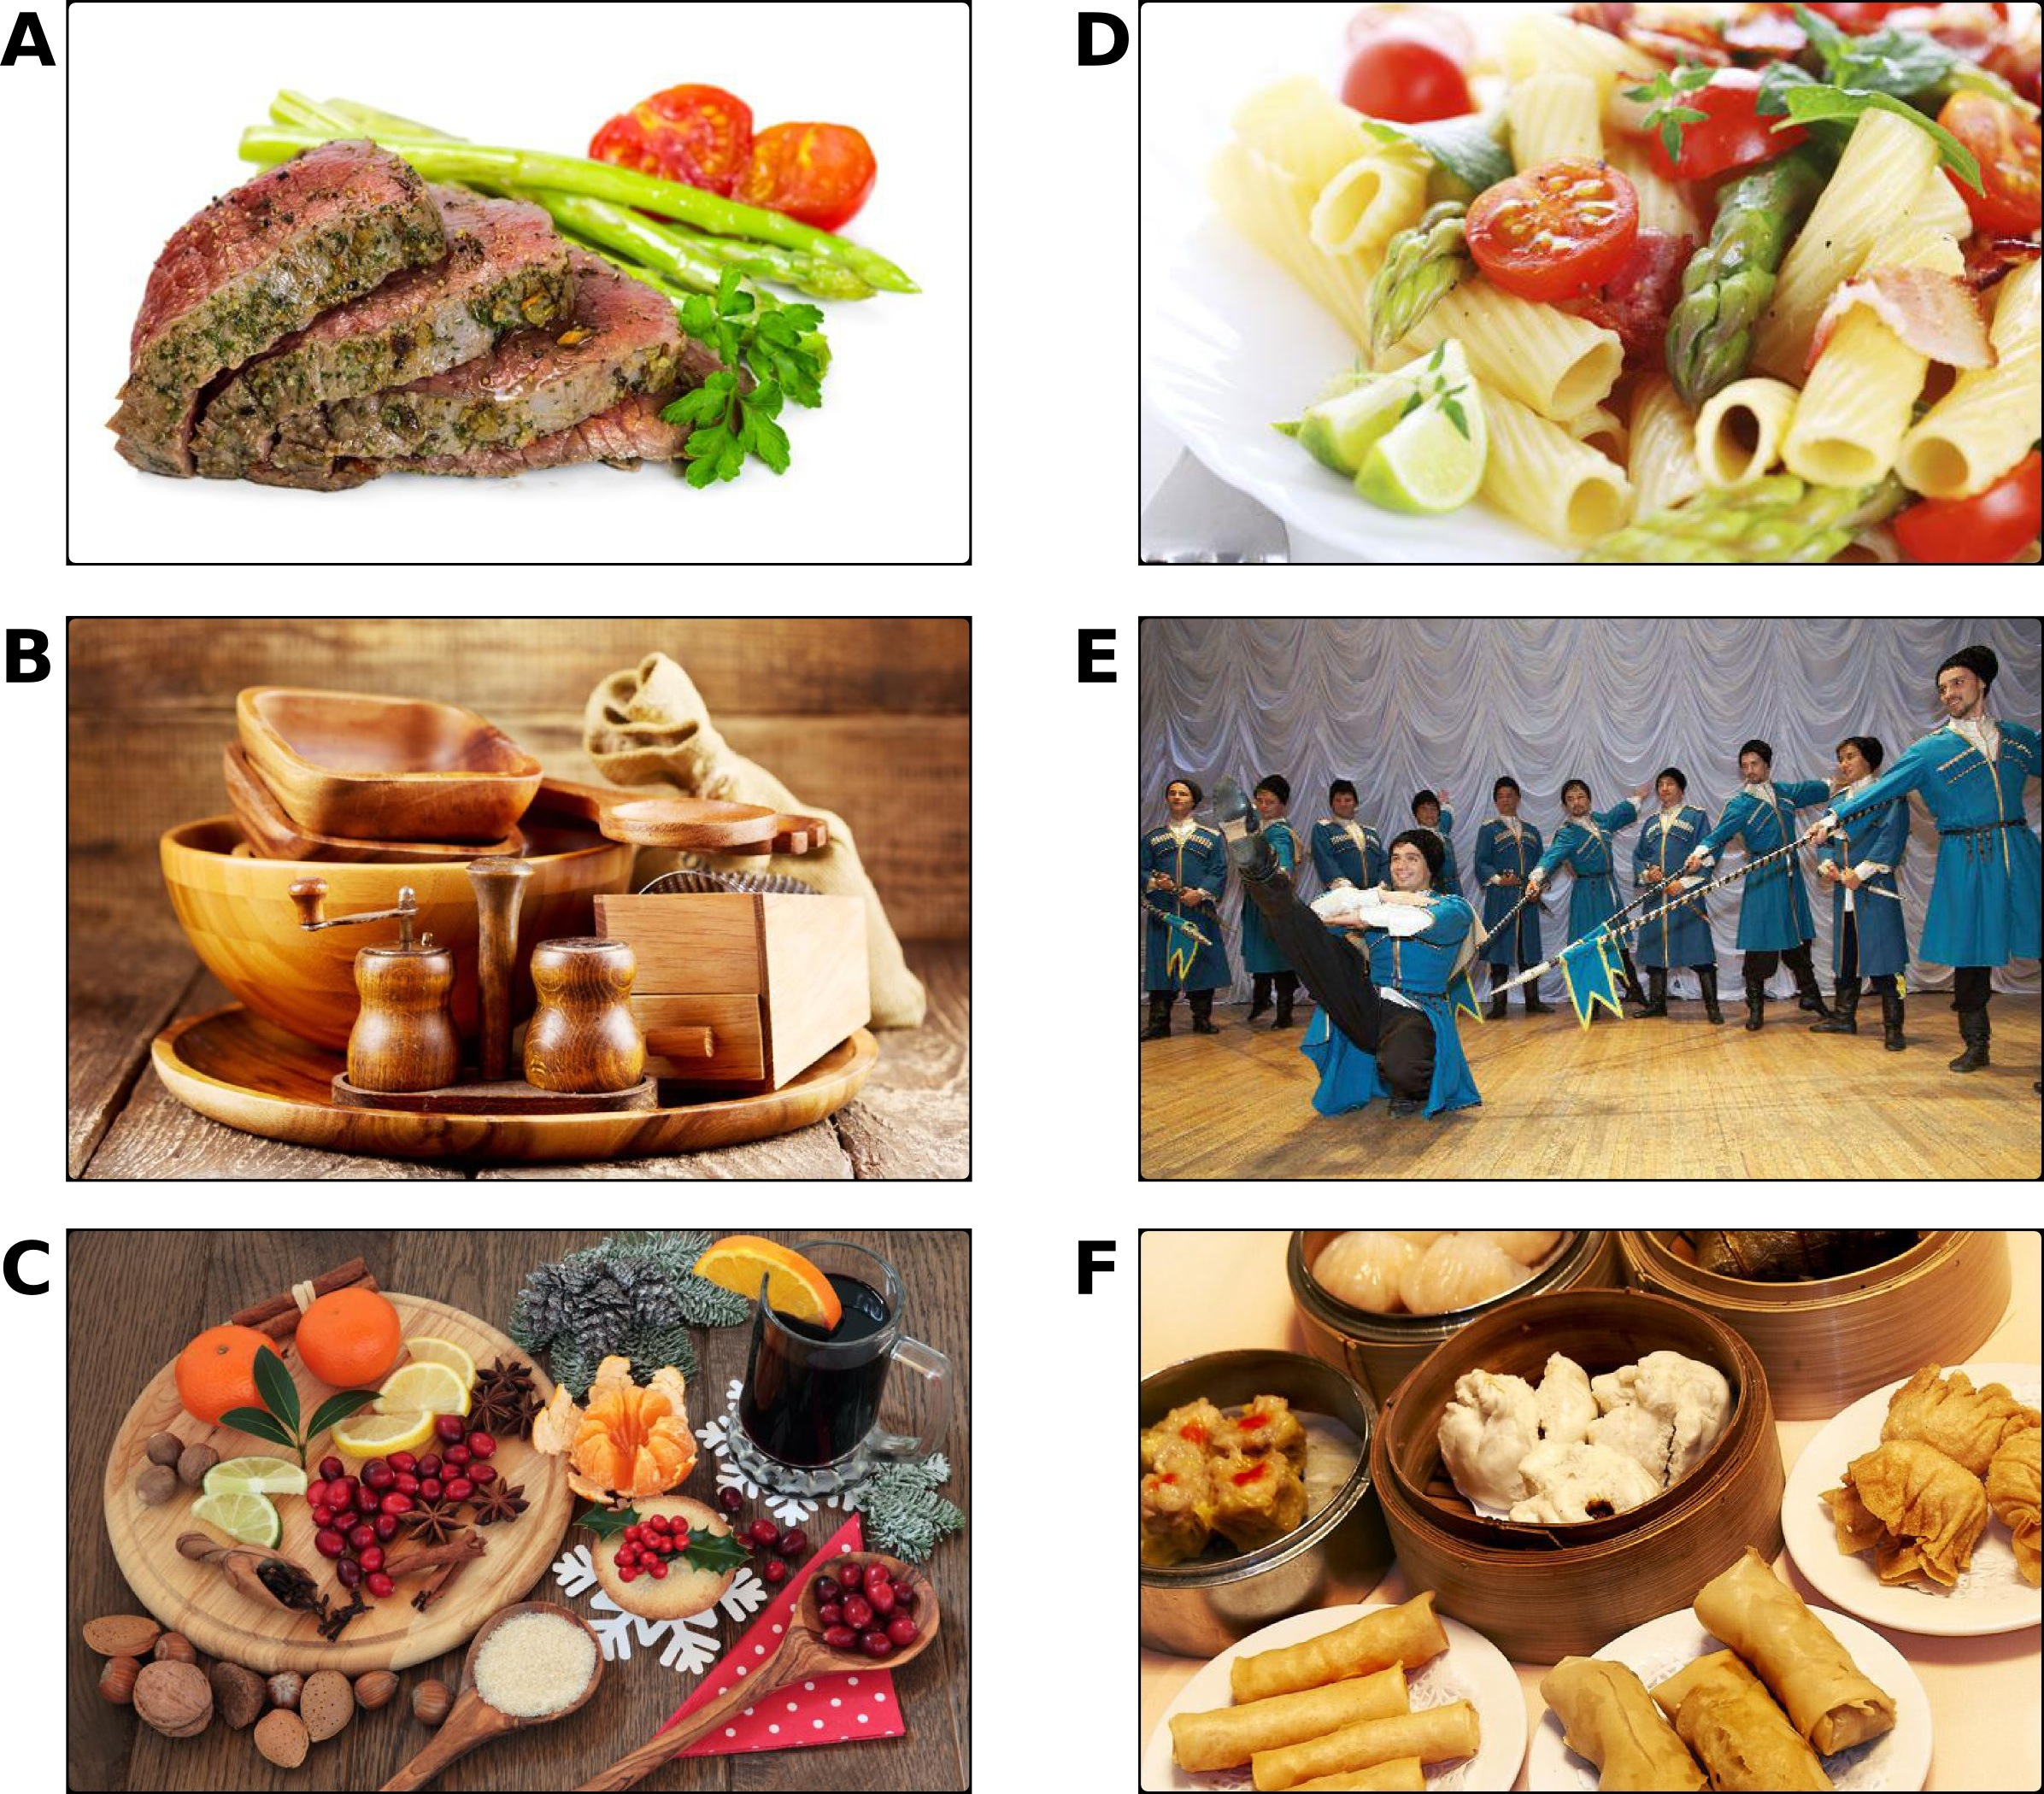
\includegraphics[scale=0.6]{figs/images.pdf}
	\caption{
		Examples of images used for various experiments and treatments:
		(A) initial task for \textit{task1:food}, (B) initial task for 
		\textit{task1:obj}, (C) test task for treatments in \textit{exp1}, 
		(D) initial task for \textit{task2:food}, 
		(E) initial task for \textit{task2:cult},  
		(F) test task for treatments in \textit{exp2}.  
		The full set of experimental materials is shown in the 
		supplementary text.
	}

	\label{fig:task}
\end{figure}

%\setlength{\tabcolsep}{2pt}
%\begin{table}[t]
%\centering
%\begin{tabular}{ c c c c c }
%		\hline \noalign{\smallskip}
%		\multicolumn{3}{c}{\textbf{Treatment name}} & \parbox[c]{1.4cm}{\centering \textbf{Frame}} & \parbox[c]{1.3cm}{\centering \textbf{Initial\\ tasks}}	\\ 
%
%		\noalign{\smallskip} \hline \noalign{\smallskip}
%
%		\multirow{6}{*}{ \parbox[c]{0.8cm}{ \phantom{XX} exp1}} 
%			& \multirow{2}{*}{task1} & food & none & food\\
%			& & obj & none & objects\\
%
%			\noalign{\smallskip} \cline{2-5} \noalign{\smallskip}
%			& \multirow{2}{*}{frame1} & food & food & none\\
%			& & obj & objects & none\\
%
%			\noalign{\smallskip} \cline{2-5} \noalign{\smallskip}
%			& \multirow{2}{*}{echo1} & food & food & none\\
%			& & obj & objects & none\\
%
%		\noalign{\smallskip} \hline \noalign{\smallskip}
%
%		\multirow{4}{*}{\parbox[c]{0.8cm}{exp2}} 
%			& \multirow{2}{*}{task2}  &  food & none & food\\
%			& 	&  cult & none & culture\\
%			\noalign{\smallskip} \cline{2-5} \noalign{\smallskip}
%			& \multirow{2}{*}{frame2} & food & food & food\\
%			& 	& cult & culture & food\\
%
%		\noalign{\smallskip} \hline  
%	\end{tabular}
%
%	\caption{ 
%		We use the treatment names shown to refer to specific sections of 
%		the experimental data.
%	}
%	\label{table:treatments}
%\end{table}

Using a na\"ive Bayes classifier (\# in the 
supplementary material we discuss the choice of classifier, the
approach to measuring accuracy, and draw a comparison to the results obtained 
if a support vector machine is used.), we found a bias of 30\% between 
workers from the \textit{food} and \textit{objects} treatments, due to 
intertask effects.
As a point of comparison, we performed a similar experiment in which we 
framed the purpose of the tasks.  Workers were either told that the tasks 
were ``Funded by the laboratory for the visual perception of Food and 
Ingredients'', or ``\ldots of Objects and Tools''.  We estimated the bias 
induced by framing using a na\"ive Bayes classifier, but did not find a 
statistically significant effect (see Fig.~\ref{fig:theta}).  This suggests
that prior task exposure is a stronger priming modality than framing.

We conducted variants of these experiments using different images, to see 
whether this trend was robust.  In the experiment 
\textit{intertask-food-culture},
workers were either assigned to a \textit{food} or \textit{culture} treatment.
As before, the initial tasks for the \textit{food} treatment contained images 
depicting food (\#) (see Fig.~\ref{fig:task}D). 
In the \textit{culture} treatment, 
the initial tasks contained images depicting cultural scenes 
(of dance, sport, or music) (see Fig.~\ref{fig:task}E).  The test tasks, which were identical for both
treatments, included images depicting meals of identifiable cultural 
origin 
(see Fig.~\ref{fig:task}F).  Results for this experiment again showed a 
strong bias (about 50\%; see Fig.~\ref{fig:theta}A) between the labels 
provided by workers from the two 
treatmens during test tasks.  Again, we compared intertask effects to framing,
by performing an experiment (\textit{frame-food-culture}) using 
the same test tasks as in \textit{intertask-food-culture}, in which we exposed
workers to a statement framing the purpose of the tasks as the recognition 
of either food or cultures.  
For this framing experiment, we did not observe a statistically significant 
difference between the labels attributed by the \textit{food} and 
\textit{culture} treatments during test tasks (see Fig.~\ref{fig:theta}).

It was only when we combined the use of framing, with an active 
reiteration step, that bias reached a level comparable to that achieved 
by intertask effects.  In the experiment \textit{echo-food-objects},
after framing the purpose of the task around either the recognition of food
or objects, we required the worker to echo back the purpose of the task
using combo-box input.  In this case, workers exposed to different 
``echoed framing'' showed a bias of about 35\% in the labels provided during 
test tasks
(see Fig.~\ref{fig:theta}A). However, it is possible that by requiring 
workers to reiterate the language used in framing, we provided an implicit 
but nonetheless strong signal that the worker must act on the framing 
statement.  In this sense, \textit{echo-food-culture} may reflect the 
influence of an instruction rather than framing.

\begin{figure}
	\centering
	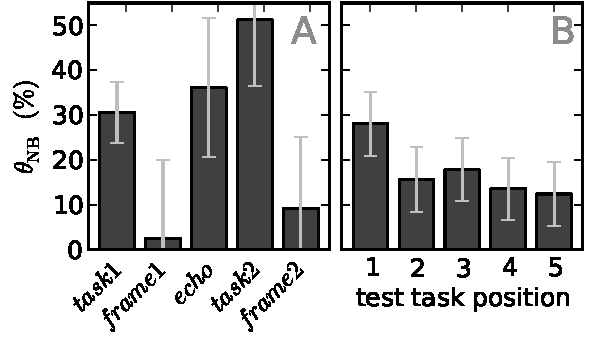
\includegraphics[scale=1]{figs/theta.pdf}
	\caption{
		Bias as measured by a na\"ive Bayes classifier, $\theta_\mathrm{NB}$,
		induced in image-labeling tasks, due to framing and 
		intertask effects. 
		(A) Bias in the responses to five test tasks,
		measured between the pairs of treatments indicated on the abscissa.  
		(B) Bias between the treatments of \textit{task1}, 
		measured for individual test tasks, and plotted as a function of 
		task position.  Error bars show the 95\% confidence intervals.
	}
	\label{fig:theta}
\end{figure}

\begin{figure}
	\centering
	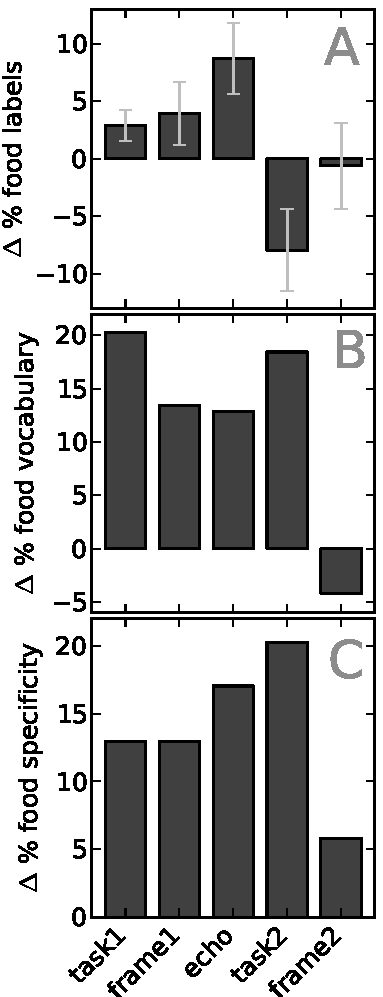
\includegraphics[scale=1]{figs/vocab_specificity.pdf}
	\caption{
		Intertask and framing effects on the vocabulary workers use to refer 
		to food(\#), when labeling images, for various treatment pairs.
		(A) Relative change in the number references to food. 
		(B) Relative change in the number of \textit{unique} 
		references to food (lexical richness). 
		(C) Relative specialization of food references, based on the 
		hypernym-hyponym relations (this calculation is shown in the 
		supplementary text).  For all
		plots, a positive bar height indicates that the \textit{*:food}
		treatment has more of the quantity than its conjugate treatment.
	}
	\label{fig:specificity}
\end{figure}

To better understand the nature of the 
intertask effects, we investigated the vocabulary
that workers used to label test tasks. A natural expectation is that, within
a given experiment, the food-primed workers would use more food-related words 
than their non-food-primed counterparts.  However, this was not generally 
the case. In the \textit{intertask-food-culture} experiment, food-primed
workers actually used significantly \textit{fewer} food-related words 
during test tasks
(\# food related words were identified using the wordnet corpus, augmented
with additional words obtained by crawling a recipe website (see supplementary
information for details)) (see Fig.~\ref{fig:specificity}).  This finding
rules out a simplistic conception of how intertask effects guide the worker's
attention.  It seems that when workers encounter content in 
prior tasks, the probability that they will refer to similar content in 
test tasks changes significantly, although it does not necessarily increase.

To clarify this observation, we investigated workers' lexical richness in 
reference to food, that is, the number of \textit{unique} food-related words
used.
Both \textit{intertask} experiments showed that food-exposed workers had 
greater lexical richness, in reference to food, than their non-food-primed 
counterparts (as much as 20\% more; see Fig.~\ref{fig:specificity}).  This
held in the case of \textit{intertask-food-culture}, even though, in that 
experiment, food-primed workers referred to food less often overall.  
This enrichment of the food-related lexicon 
was also observed in the \textit{priming-food-objects}, and 
\textit{echo-food-objects} experiments, but to a lesser extent.

This suggests that priming, by prior task exposure as well as framing,
might have led workers to use more refined or specialized words to refer to
the concept present in the prime.
To test this directly, we used the wordnet corpus to operationalize the 
notion of word specialization.
Wordnet provides a set of hypernym-hyponym relations between \# English 
nouns.  
Hypernyms are generalizations (for example, ``bread'' is a hypernym for 
``pumpernickel''), while hyponyms are specializations.
To assess the relative specialization of words from two different treatments,
we compared all pairs of words from one treatment to the other. 
We tallied the cases where a word from one treatment was more specialized
than one from the other, as well as the cases with roles reversed.  
The difference of these tallies, as a percentage of their total, gave the
relative specialization of one treatments vocabulary over the other
(\#) (see Fig.~\ref{fig:specificity}).  
Using this approach, we compared the specialization of food-related words 
for the treatments of all experiments.

In all experiments except \textit{frame-food-culture}, food-primed workers 
used significantly more specialized words than their non-food-primed 
counterparts (about 15\% more; see Fig.~\ref{fig:specificity}C).
It is interesting that such substantial increases in both the lexical 
richness and specialization of food-related words among food-primed workers
held for \textit{intertask-food-culture}, where, again, we observed fewer 
references to food by food-primed workers overall. These observations point 
to countervailing factors: one tending to activate the more specialized and 
less common food-related words (yielding greater lexical richness and 
specialization), and the other tending to suppress certain, presumably more 
common or generic words (yielding fewer food-related words in total).

This hypothesis is corroborated when we look at those words whose 
frequencies changed the most from one treatment to another (see Table S1).  
The word ``food'', which is the most generic possible food-related word, was 
always \textit{suppressed} among food-primed workers.  In fact, 
for all experiments, ``food'' was the \textit{most suppressed} word.

Taken together, our results can be 
explained through a combination of positive and negative priming.
Positive priming (usually simply ``priming'') occurs when a prior stimulus 
predisposes a person to give certain responses in an ensuing task, and
is often observed as an increase in the speed or accuracy of a response, or
the ability to recognize features of a briefer, quieter, or noisier stimulus 
(\#).
Negative priming occurs when, after being repeatedly exposed to a stimulus 
considered to be non-salient, a person begins to ignore that 
stimulus (\#).  

Workers exposed to images containing food will be (positively) primed, 
activating memories, concepts, and vocabulary related to food.  
However, as the worker labels successive images containing food, the basic 
fact that an image contains food will not appear to be salient, since it 
does not serve to distinguish one image from another.  Thus, the most 
generic references to that fact, such as the label ``food'', 
will be suppressed, while more specialized references will be elicited.  
Meanwhile, the number of references to food overall might increase or 
decrease, depending on the balance of these factors.  

More generally, we are suggesting that, even though workers are not 
instructed to compare tasks in any way, prior tasks form a 
context relative to which workers judge salience.  Thus, due to a combination 
of negative and positive priming, a worker's focus 
in repeated tasks tends to be directed away from generic, shared features, 
toward specific and distinguishing ones.

Prior to this study, little thought appears to have been given to the 
ordering and bundling of tasks.  But our findings show that these are 
powerful design factors.  A natural response to our findings 
might be simply to randomize task ordering, a practice that is commonly 
observed.  But the sheer extent of bias that we observed leads us to question 
whether that is the best approach, since this would tend to raise 
the ``noise floor'' of the study.

Furthermore, our findings suggest that, through careful task engineering,
it might be able to achieve much more.  The boost that we observed to the 
specialization and richness of workers' responses motivates further 
investigation to acquire a deeper understanding of intertask effects.  
We hope that future work will yield techniques to leverage intertask effects, 
enabling one to tune the focus, diversity, and specialization of worker 
responses.

A consistent goal in human computation is the achievement of expert-level
judgments from non-expert workers.  This has been achieved in some
applications (\#). The distinction between experts and novices can be 
attributed in part to the knowledge of facts and 
heuristics. But to a large degree, this distinction lies in the ability of 
experts to direct their focus towards salient features, while filtering out 
non-salient ones \cite{kellman2009perceptual}.  Using prior task exposure to 
guide focus and salience attribution might well enable expert-level 
judgment in a wider variety of crowdsourced applications.

Here we have shown that a large bias can be introduced into microtask 
responses, simply from the performance of earlier tasks. 
These effects are much stronger than framing, and are only comparable when
framing is combined with a requirement that the worker actively echo
the framing language.  While our findings raise serious concerns about the 
current state of microtask design, it also reveals opportunities for more 
refined control over worker focus and acuity.  Any application that relies
on the repetitive use of human judgment is likely subject to the phenomena
we described here.  It remains to be determined whether intertask effects 
can be leveraged to increase the performance and reliability of human 
computation.

\bibliography{newbib}
\bibliographystyle{Science}


\section*{Supplementary Material}

\subsection*{S1: Experimental materials}
The tasks for both experiments were presented as a series of slides.  In
both cases, the first slide consisted of a brief set of instructions, followed
by the frame if shown (only some treatments involved a frame), see 
Fig. S\ref{fig:hit_preamble}.  Following the instructions and prime, a set
of initial tasks was shown (except for the treatments in \textit{frame2}
and \textit{echo1}) followed by (in all cases) a set of test tasks.  In
\textit{exp1}, two kinds of frame were used, one simple frame, and one where
the worker was required to echo the frame using a combo-box input.  The
instructions, both kinds of frame, and an example task slide, are shown 
in Fig. S1.
\begin{figure}
	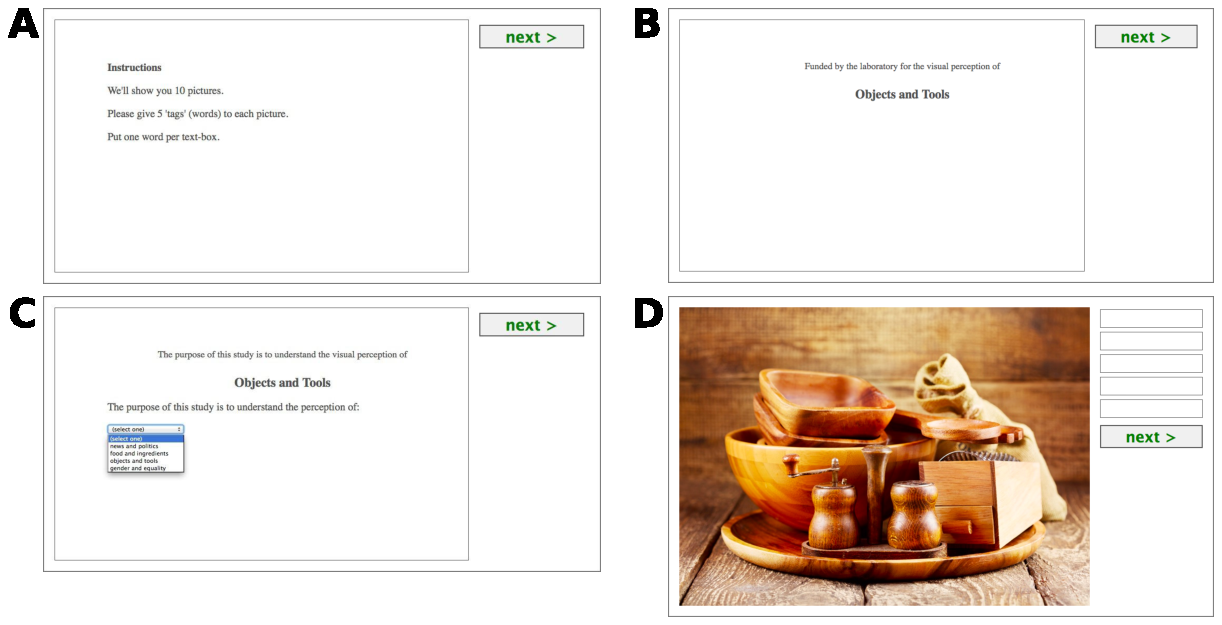
\includegraphics[scale=0.8]{figs/tasks.pdf}
	\label{fig:hit_preamble}
	\caption{Examples of A) instructions; B) a frame, as shown in 
		\textit{frame1:obj}, and similar to those shown in 
		\textit{frame1:food} and \textit{frame2:food}, and 
		\textit{frame2:cult};  
		C) an echoed frame, as used in \textit{echo1:obj}, and similar to that
		used in \textit{echo1:food}; and D) an 
		example of an image-labeling task.
	}
\end{figure}

All of the initial tasks had the format shown in Fig. S1D.  The images used
in the initial tasks for \textit{task1:food} and \textit{task1:obj} are
shown in Fig. S2 and S3, and the images used in the test tasks for 
\textit{exp1} are shown in Fig. S4.  The images used in the initial tasks
for \textit{task2:food} and \textit{task2:cult} are shown in Fig. S5 and
Fig. S6 respectively, and the images used in the test tasks for \textit{exp2} 
are shown in Fig. S7.

\begin{figure}
	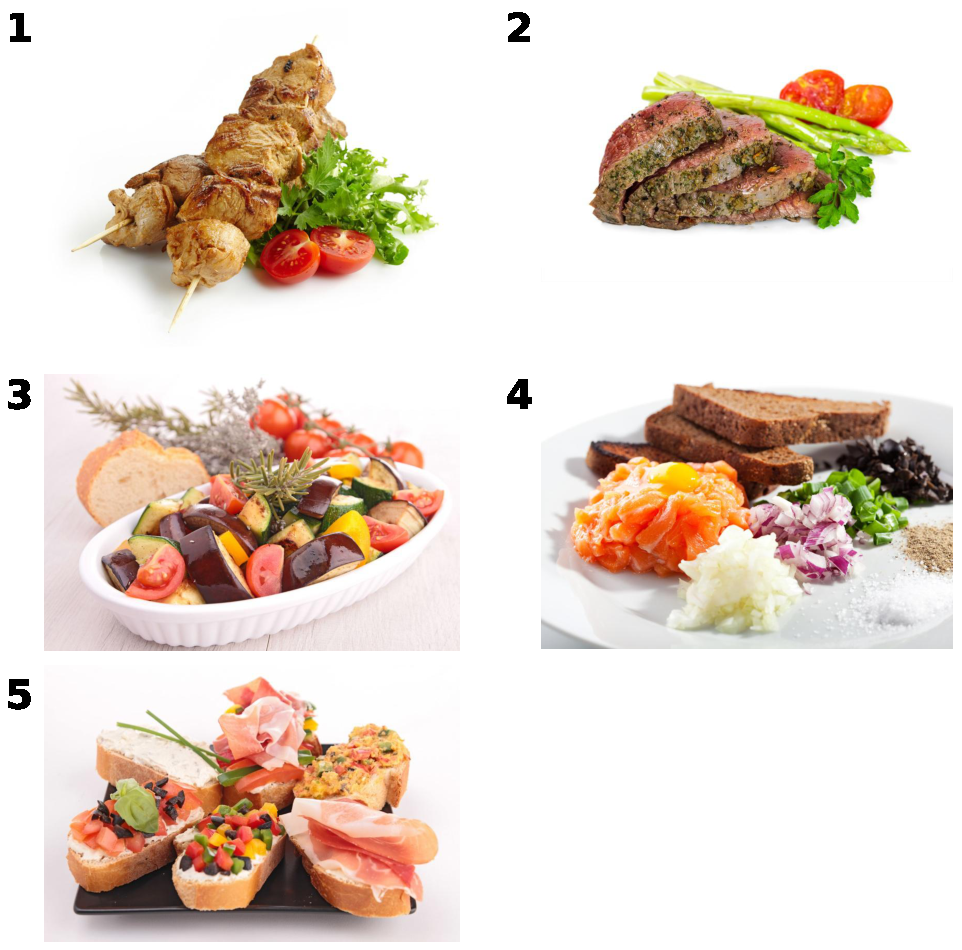
\includegraphics{figs/task1-food.pdf}
	\label{fig:task1:food}
	\caption{
		Figure S2: Images used in the initial tasks for 
		\textit{task1:food}.  The numbers show the order in which the 
		images were presented to workers.
	}
\end{figure}

\begin{figure}
	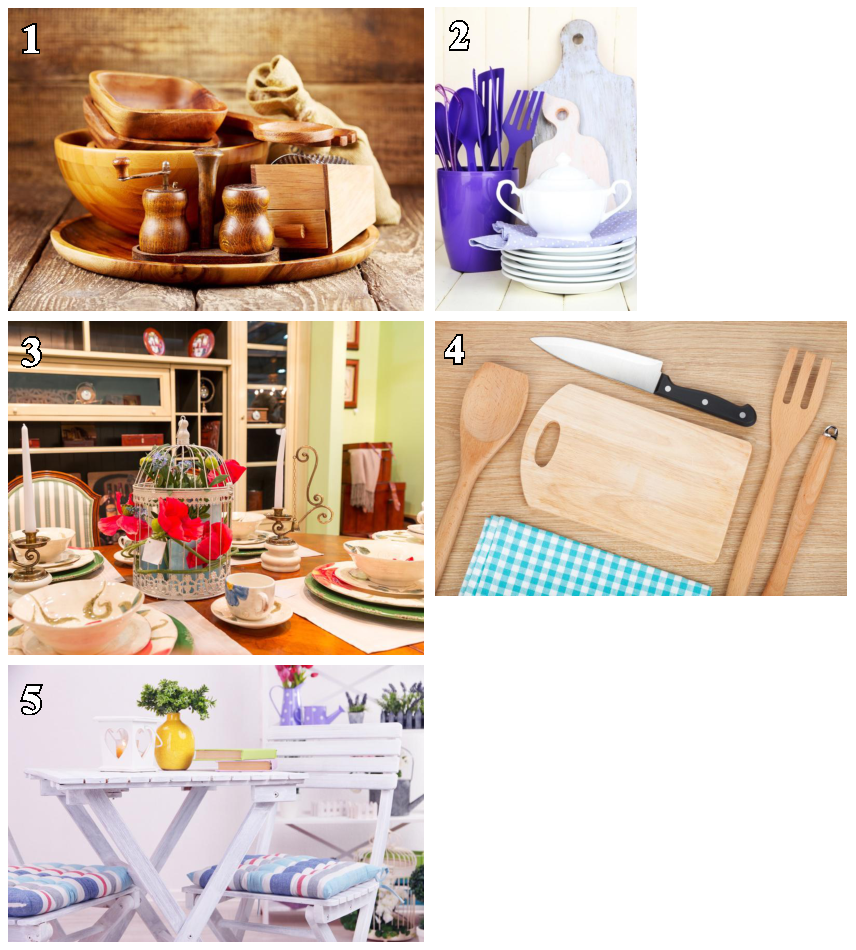
\includegraphics{figs/task1-obj.pdf}
	\label{fig:task1:obj}
	\caption{
		Figure S3: Images used in the initial tasks for 
		\textit{task1:obj}.  The numbers show the order in which the 
		images were presented to workers.
	}
\end{figure}

\begin{figure}
	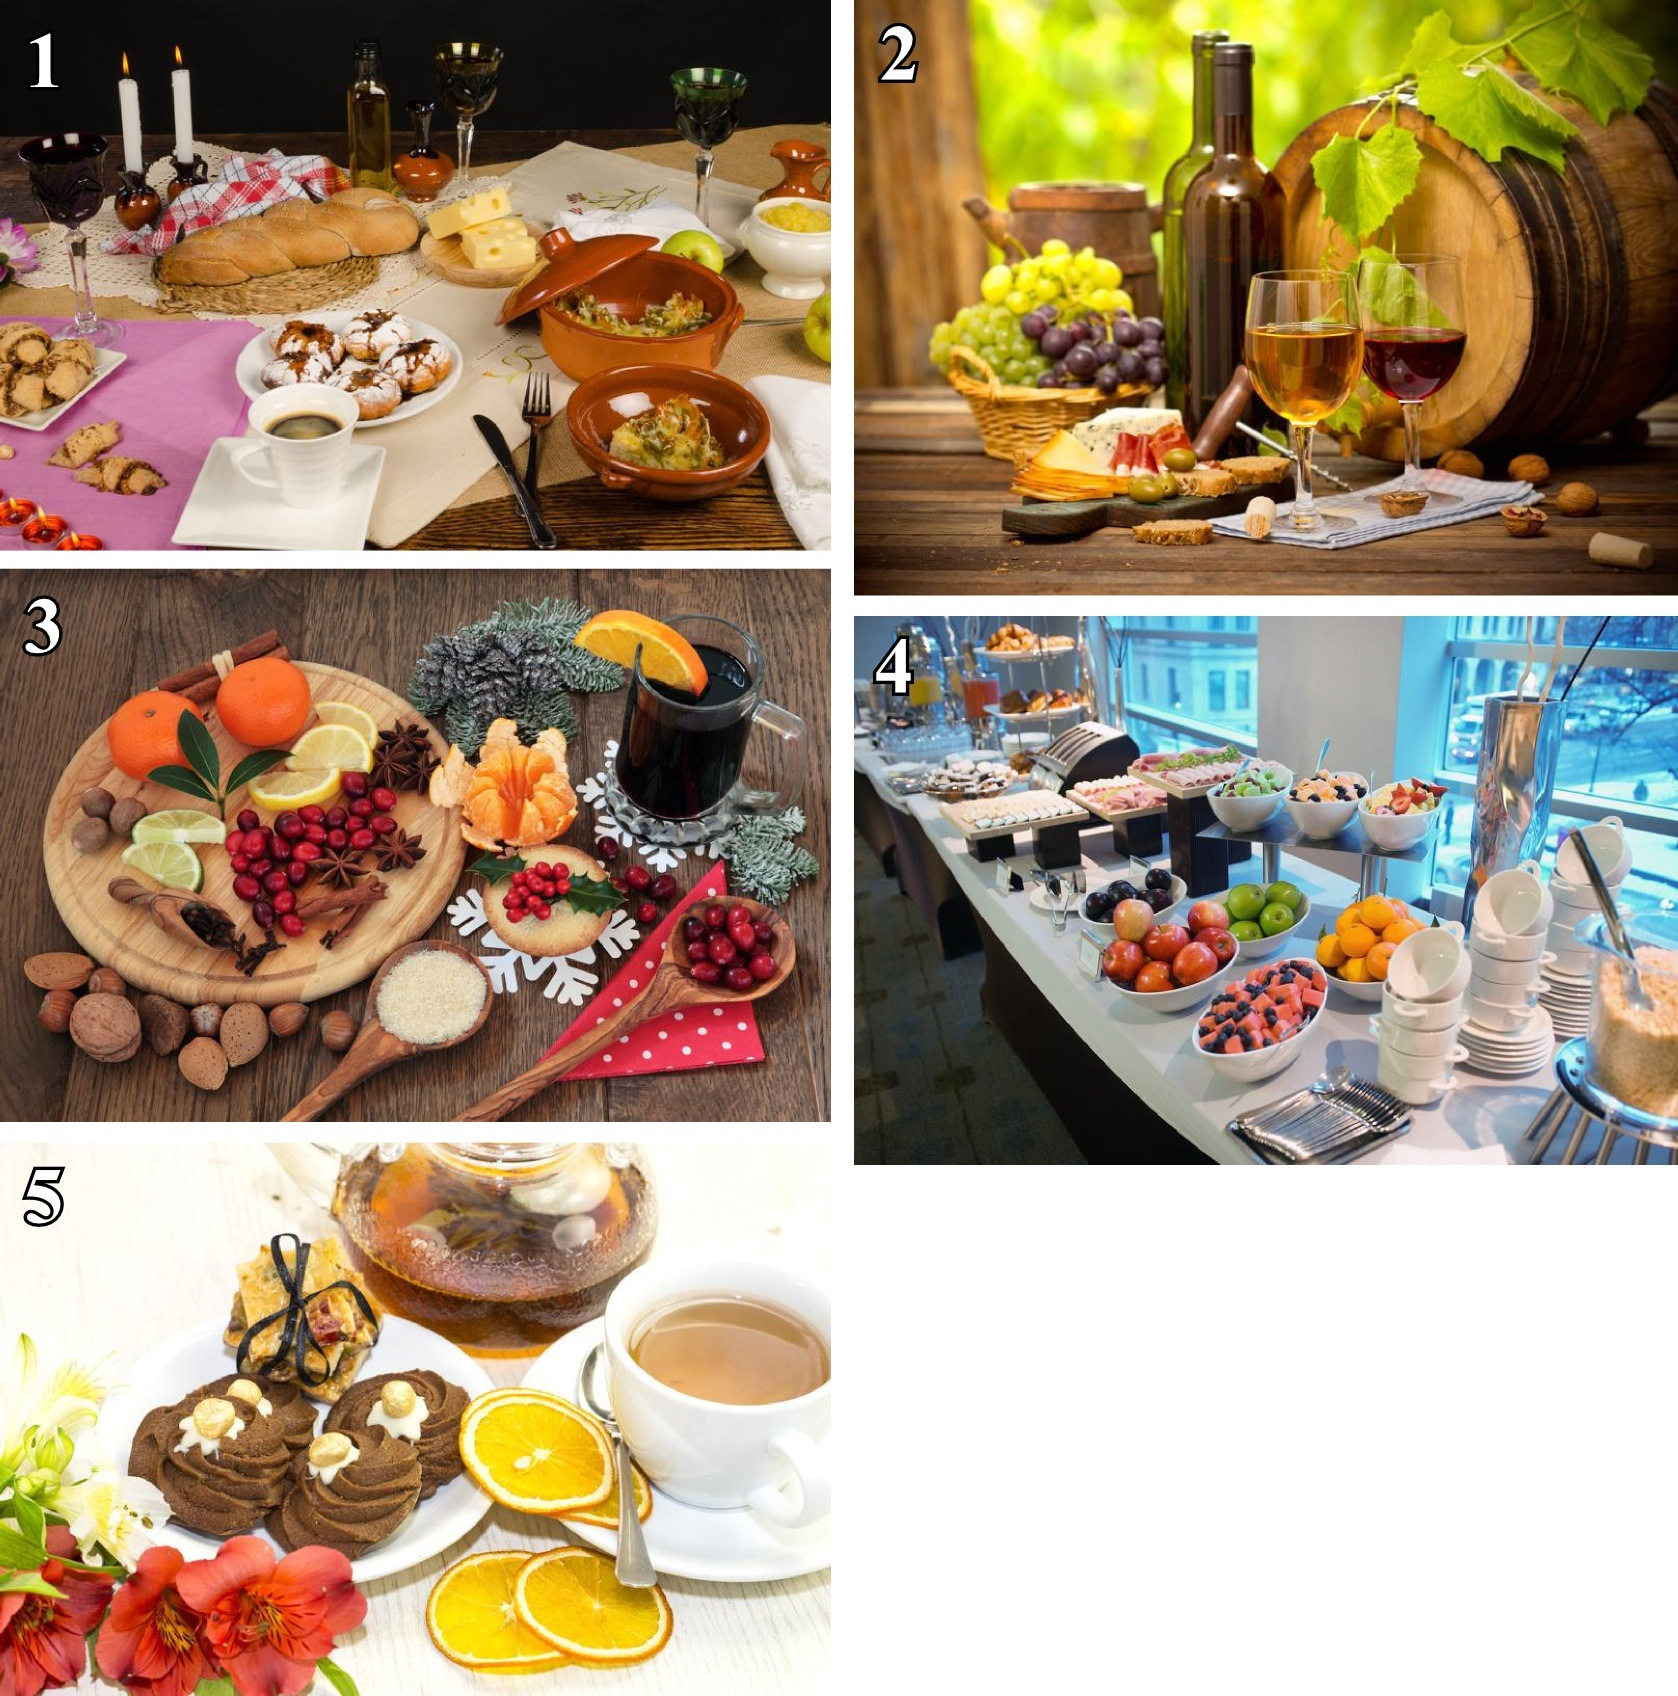
\includegraphics{figs/task1-test.pdf}
	\label{fig:task1:test}
	\caption{
		Figure S2: Images used in the test tasks for 
		\textit{exp1}.  The numbers show the order in which the 
		images were presented to workers.
	}
\end{figure}

\begin{figure}
	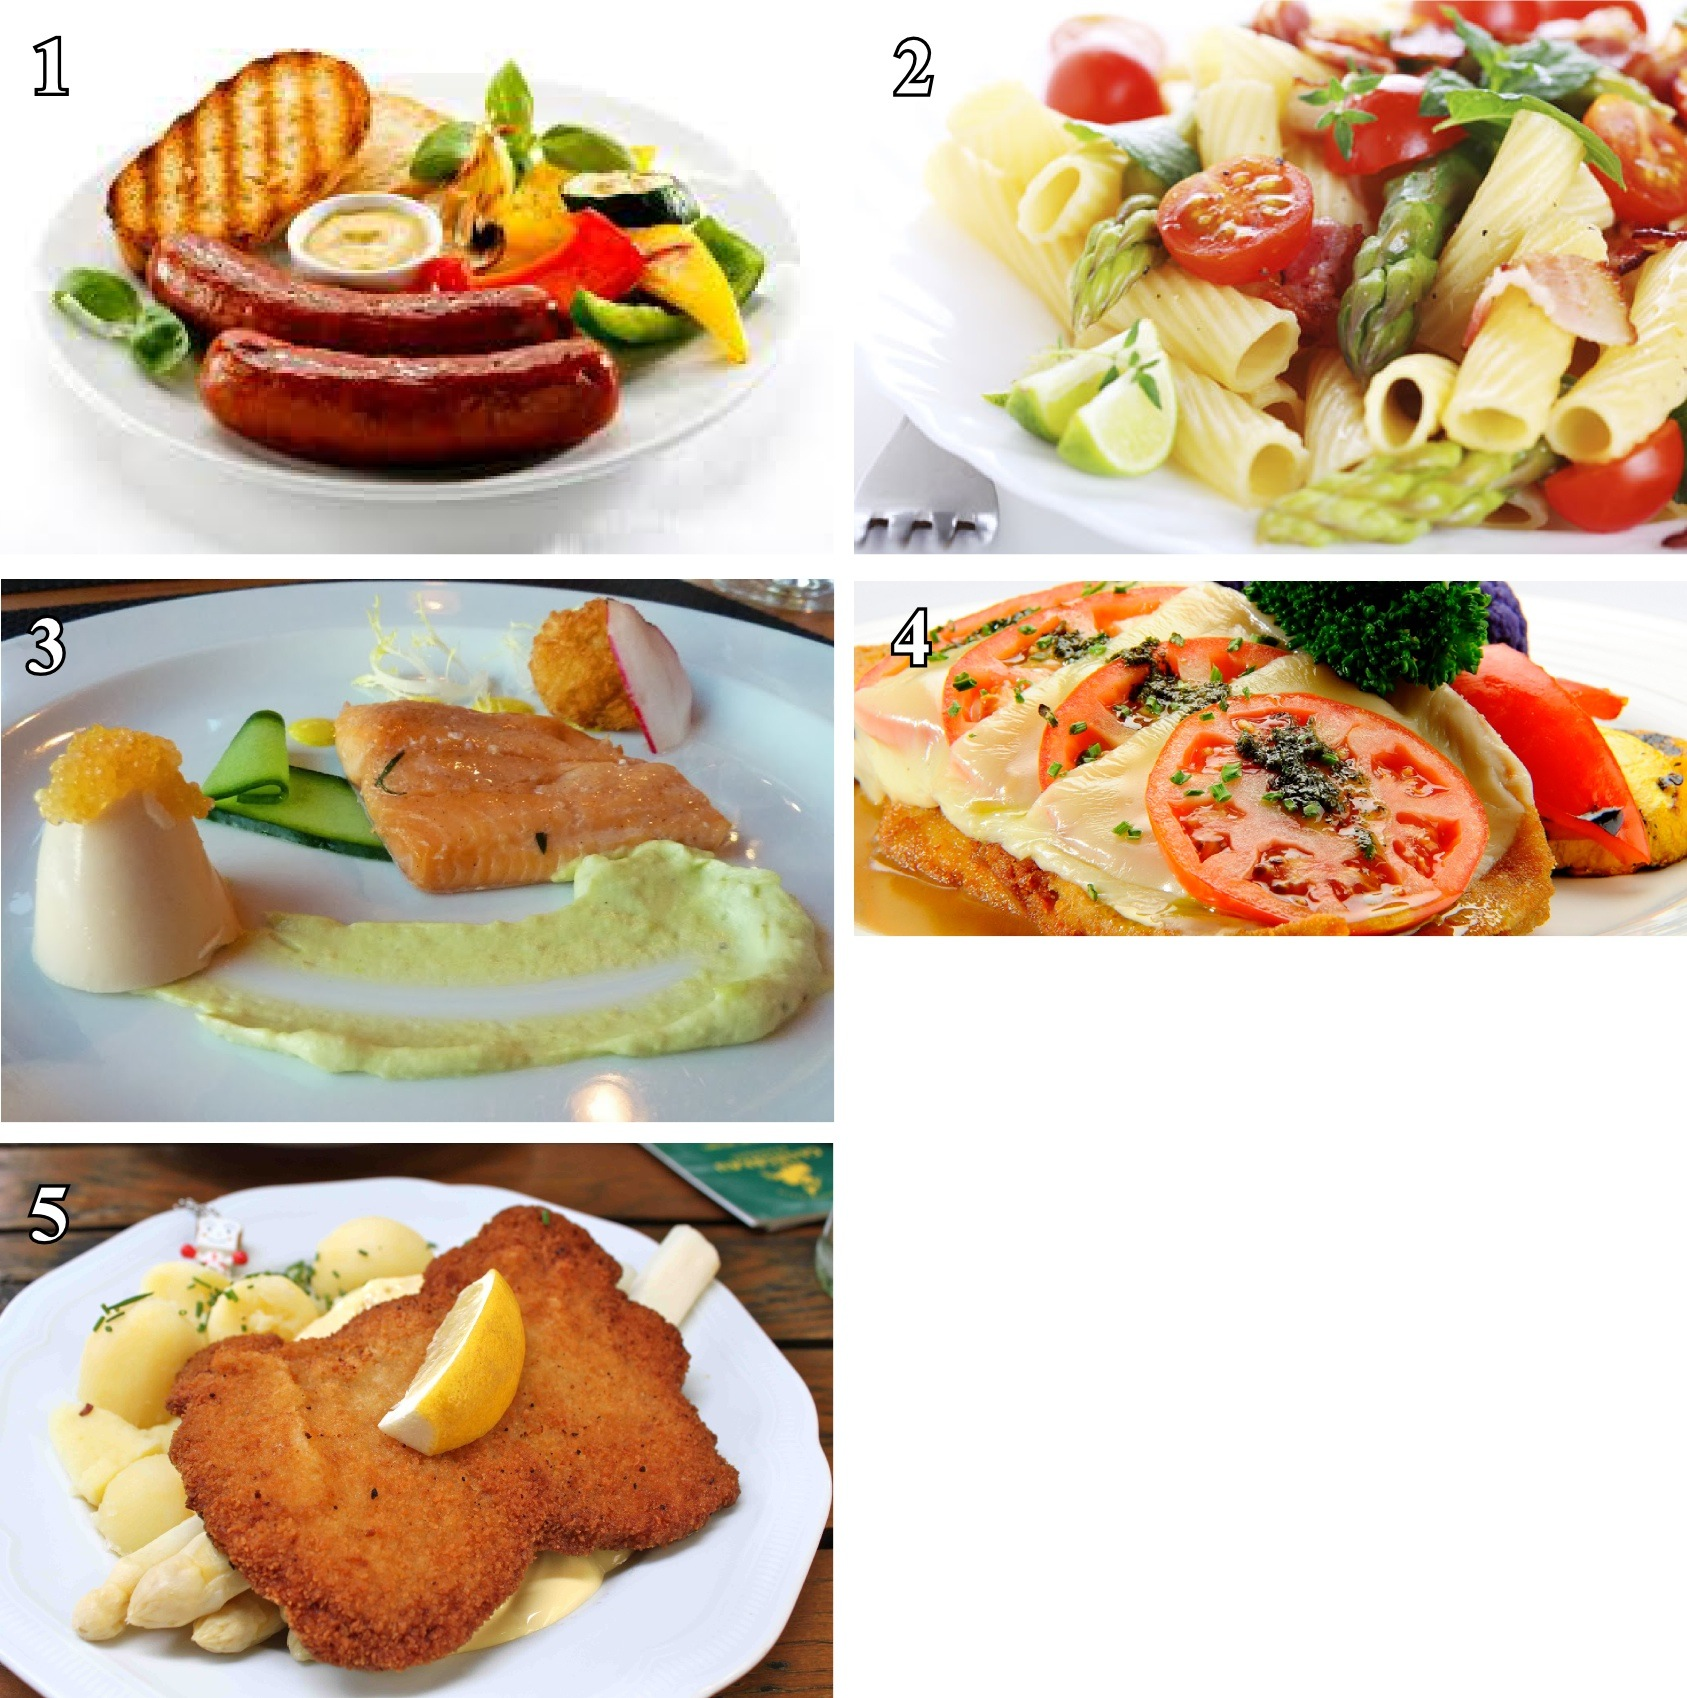
\includegraphics{figs/task2-food.pdf}
	\label{fig:task2:food}
	\caption{
		Figure S2: Images used in the initial tasks for 
		\textit{task2:food}.  The numbers show the order in which the 
		images were presented to workers.
	}
\end{figure}

\begin{figure}
	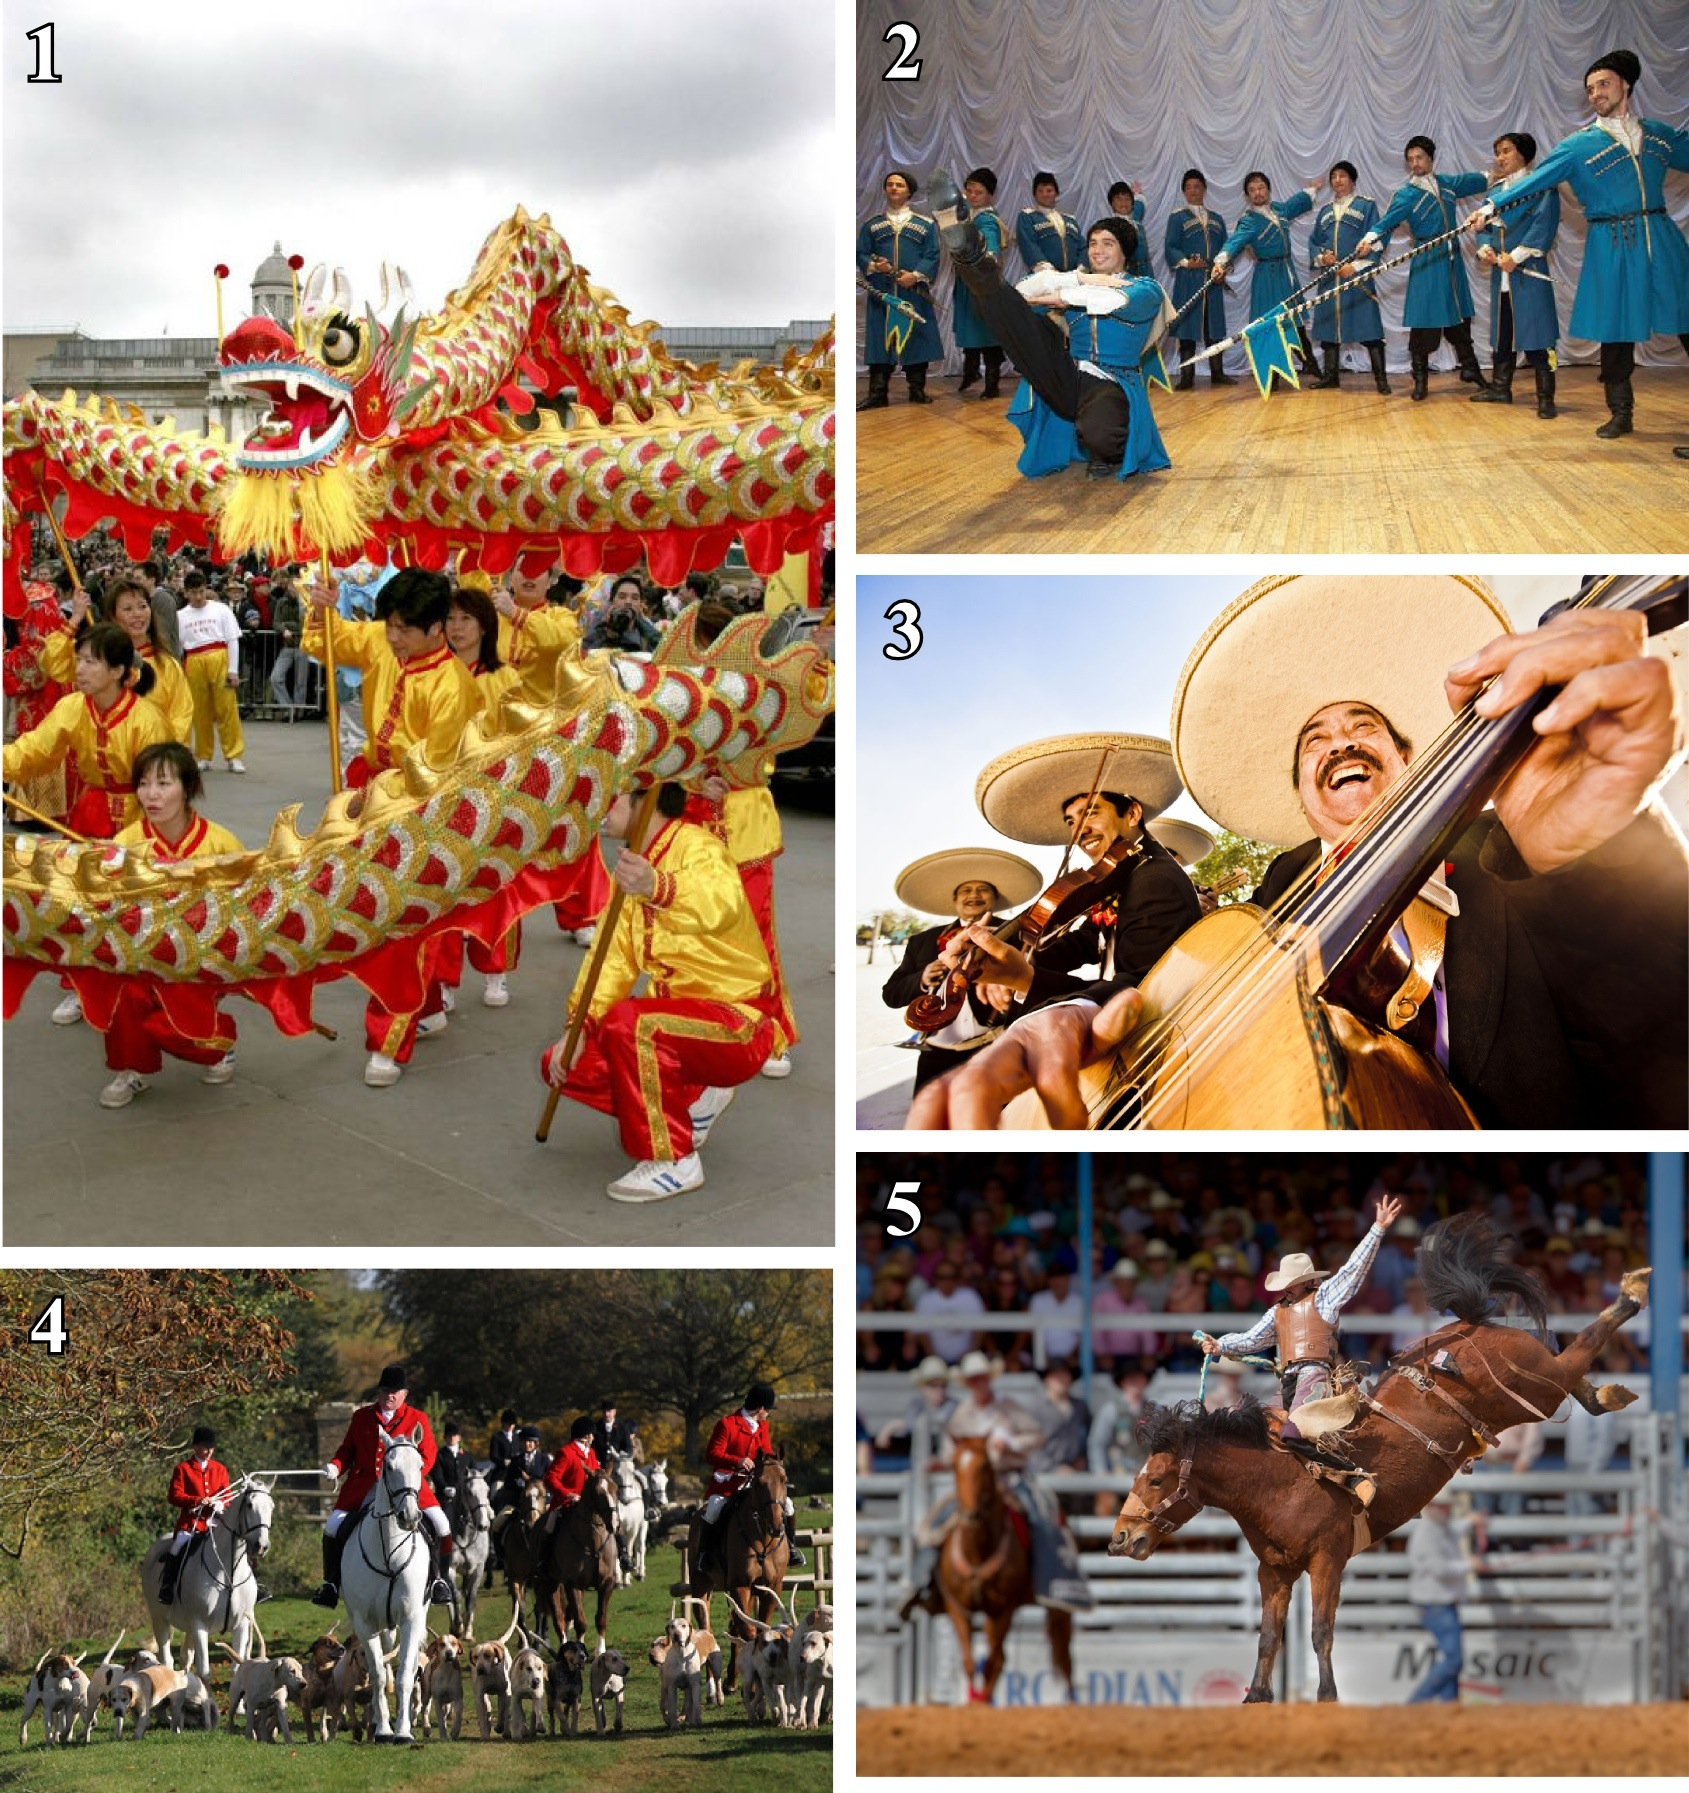
\includegraphics{figs/task2-cult.pdf}
	\label{fig:task2:cult}
	\caption{
		Figure S2: Images used in the initial tasks for 
		\textit{task2:cult}.  The numbers show the order in which the 
		images were presented to workers.
	}
\end{figure}

\begin{figure}
	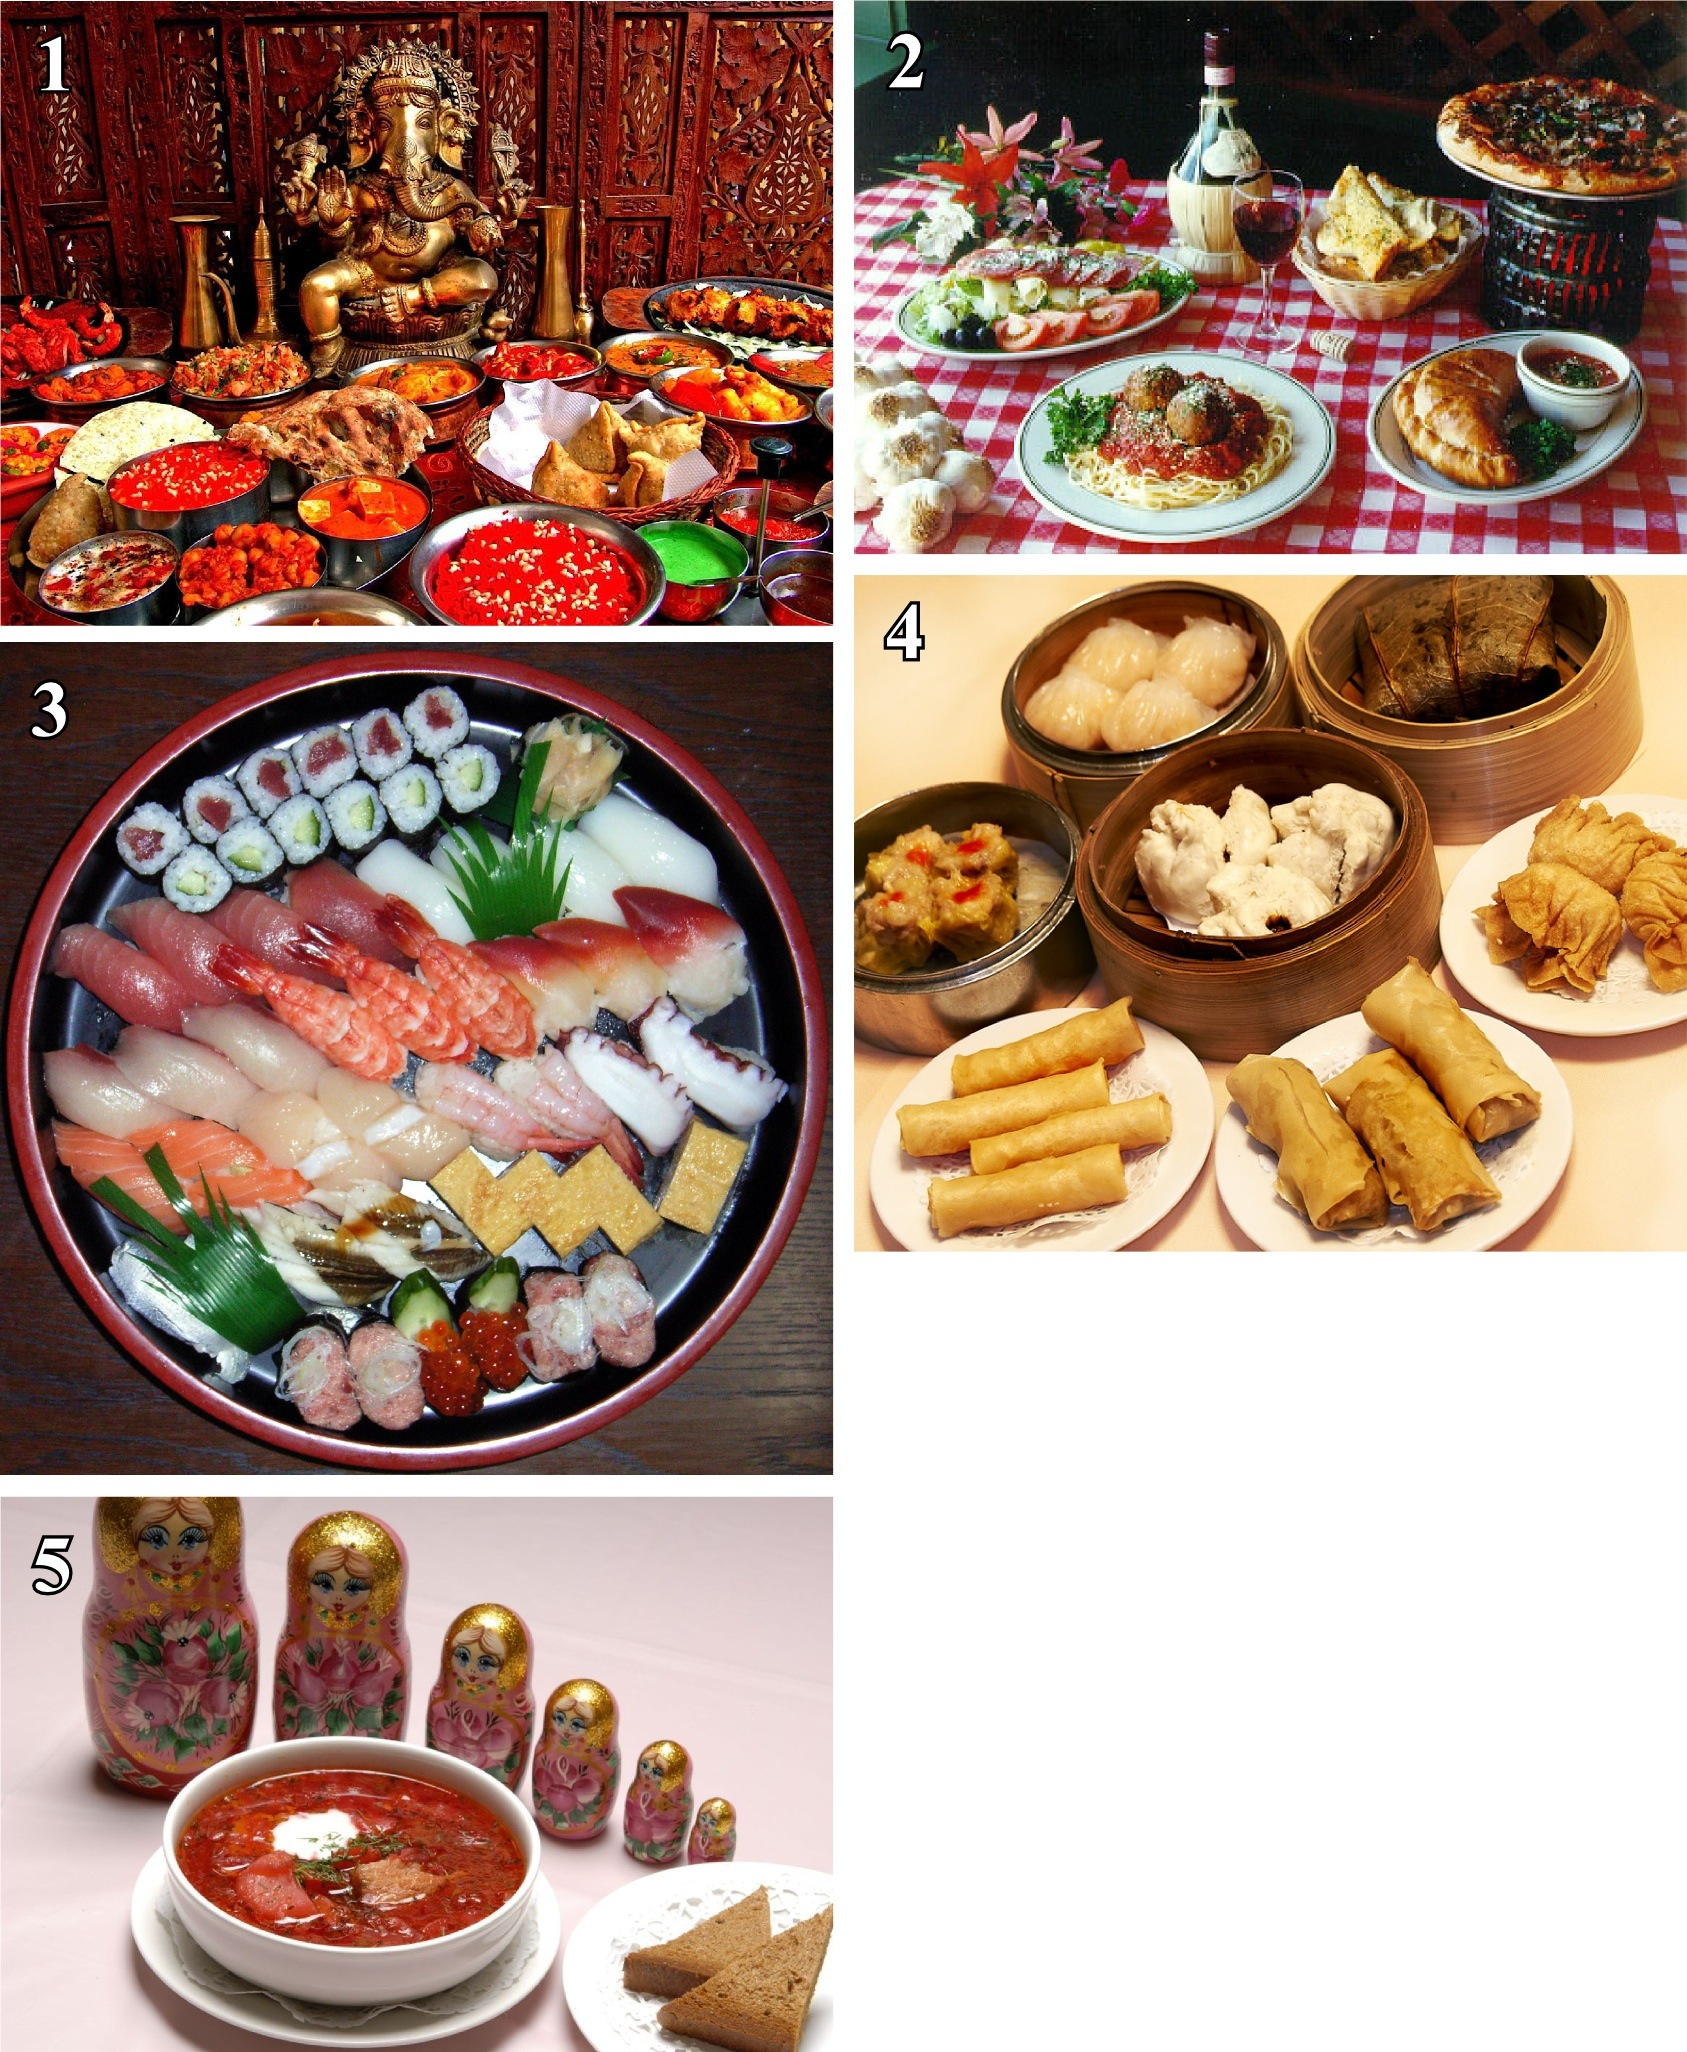
\includegraphics{figs/task2-test.pdf}
	\label{fig:task2:test}
	\caption{
		Figure S2: Images used in the test tasks for 
		\textit{exp2}.  The numbers show the order in which the 
		images were presented to workers.
	}
\end{figure}

\subsection*{S2: Access to raw data and code}
The raw data and source code needed to reproduce the analyses 
shown here and in the main text can be downloaded from 
http://networkdynamics.org/publications/public/priming2014.09.

\subsection*{S3: Additional results not shown in the main text}
		the top 5 most suppressed and most activated terms between treatment
		pairs.

\begin{table}
	\centering
	\setlength{\tabcolsep}{10pt}
	\begin{tabular}{ c c c c c }
	
		\setlength{\tabcolsep}{4pt}
		\begin{tabular}{ r | c }
		\toprule
		\multicolumn{2}{c}{\textit{task1}} \\
		\toprule
		coffee & 38 \\
		meal & 34 \\
		cheese & 34 \\
		apple & 32 \\
		dessert & 21 \\
		cup & -30 \\
		glass & -45 \\
		table & -70 \\
		candle & -74 \\
		food & -80 \\
		\bottomrule
		\end{tabular}

&

		\setlength{\tabcolsep}{4pt}
		\begin{tabular}{ r | c }
		\toprule
		\multicolumn{2}{c}{\textit{frame1}} \\
		\toprule
		bread & 18 \\
		wine & 18 \\
		cheese & 16 \\
		apple & 14 \\
		oil & 12 \\
		table & -9 \\
		meal & -10 \\
		candle & -12 \\
		dinner & -13 \\
		food & -32 \\
		\bottomrule
		\end{tabular}

&

		\setlength{\tabcolsep}{4pt}
		\begin{tabular}{ r | c }
		\toprule
		\multicolumn{2}{c}{\textit{echo1}} \\
		\toprule
		apple & 24 \\
		cheese & 23 \\
		wine & 15 \\
		coffee & 14 \\
		oil & 7 \\
		knife & -24 \\
		dinner & -26 \\
		fork & -27 \\
		candle & -35 \\
		food & -55 \\
		\bottomrule
		\end{tabular}

&

		\setlength{\tabcolsep}{4pt}
		\begin{tabular}{ r | c }
		\toprule
		\multicolumn{2}{c}{\textit{task2}} \\
		\toprule
		spicy & 26 \\
		sauce & 17 \\
		indian & 15 \\
		buffet & 14 \\
		exotic & 12 \\
		festival & -11 \\
		offering & -12 \\
		statue & -15 \\
		india & -20 \\
		food & -56 \\
		\bottomrule
		\end{tabular}

&

		\setlength{\tabcolsep}{4pt}
		\begin{tabular}{ r | c }
		\toprule
		\multicolumn{2}{c}{\textit{frame2}} \\
		\toprule
		indian & 11 \\
		banquet & 8 \\
		spicy & 7 \\
		asian & 6 \\
		variety & 6 \\
		delicious & -6 \\
		meat & -7 \\
		festival & -7 \\
		spice & -7 \\
		food & -9 \\
		\bottomrule
		\end{tabular}

	\end{tabular}
	\caption{blah}
\end{table}

\subsection*{S4: Data preprocessing}
	\paragraph{Splitting, Lemmatization, removal of stop-words, and 
		addition of position tags.} 

	Before performing any analysis on the labels that workers provided, we
	performed a series of preprocessing steps.  
	\td{does this reflect the actual order in which the steps were done?}
	First, words wore lematized 
	using the
	\td{whatzit} lemmatizer.  This lemmatizer is very mild, tending only to 
	change plural words to their singular form.  Common
	words such as ``the'', ``to'', or ``with'', were found using the
	the \td{whatzit} stop-word list and removed.  Then, misspelled words were
	automatically corrected using a spelling correction algorithm described 
	below.  Finally, labels that contained
	multiple words (separated by spaces or punctuation) were split, with
	punctuation removed, and the separated words were treated as distinct 
	features in subsequent analysis.

	For the purpose of training and testing a na\"ive Bayes classifier, we 
	performed an additional preprocessing step.  We tagged words with the
	position in which they had been entered (i.e. which of the five text 
	inputs in the task interface) as well as the test tasks in which the word 
	had been provided.
	So, if the word ``wine'' was entered into the second text-input for 
	the third test-task, after preprocessing, the feature ``3\_2\_wine'' would
	appear.  Prepending the task number onto words was simply a means to 
	retain correct attribution, which itself was essential since providing a
	word during one task is not equivalent to providing the same word during 
	another task.  
	
	\paragraph{Spelling correction.}  
	Spelling correction was performed using an algorithm that first detected
	if a word was likely to be misspelled, then generated a set of candidate 
	corrections, and chose the best candidate based on a scoring mechanism.
	
	A word was considered misspelled if it was not contained in the 
	\textit{legal set}, which was formed by the union of
	the wordnet corpus, the stop-word list, and a set of words seen while 
	crawling the world food section of the allrecipes.com website.  We
	describe the crawling of the allrecipes.com website in a section below.

	To correct misspellings, we first produced all possible modified forms 
	that could be obtained applying one or two edits.  An edit consisted of 
	adding or removing a letter, changing one letter into another, or 
	swapping the positions of two adjacent letters.  For the purpose of these 
	edits, spaces were treated as any other letter.

	The candidates produced by these edits which were in the legal set were
	then ranked based on a scoring mechanism, and the highest scoring word
	was chosen as the correction.  A candidate $w$'s score, $s_w$, was 
	calculated according to the following formula:
	\begin{equation}
		s_w = (f_w + 1) * p_1 * p_2,
	\end{equation}
	where $f_w$ is the frequency with which the word occurred (correctly 
	spelled)
	within the given task, $p_1$ was a penalty for the first edit, and
	$p_2$ was a penalty for the second edit.  If the word was made using only
	one edit, then $p_2 = 1$.  Any edit that did not involve adding a space
	(i.e. separating a word) incurred a penalty of 0.5, while the addition of
	a space incurred a penalty of 0.1.  Word-separation edits were more 
	strongly penalized because it is often possible to split a series of 
	letters into many short two- or three-letter words, which otherwise leads 
	to many erroneous corrections.  We found that setting the penalty for
	word splitting at 0.1 worked well by testing on words taken from
	initial tasks.

	After all of our analyses had been performed, we checked the accuracy of 
	the spelling correction algorithm using three human coders.  The coders
	were shown a set of 
	500 words that were randomly sampled from the labels attributed during 
	test tasks (50 for each test task).  Before sampling, the labels from all
	experimental treatments, for the given test task, were pooled together.
	The coders did not know which treatment any given word came from.  
	In addition to the words, coders were shown the spelling correction 
	produced by the algorithm, as well as the image from the test task.
	The coders were asked to identify any misspelled words which had not 
	been corrected, as well as any corrections that appeared to be erroneous,
	by indicating their own correction.

	Based on this exercise, we found that, according to the human coders,
	17\% of the words were misspelled, but that after applying the 
	automated spelling correction, only 3.2\% of words were misspelled.

	\paragraph{Crawling the world food section of allrecipes.com.}
	The website allrecipes.com was accessed on 3-4 November 2014 using 
	automated scripts.  A total of 2642 recipe listings and 15621 recipe
	instruction pages were crawled.  Recipe listings were pages that provided 
	lists of recipes, and contained a title and short description for each.  
	The recipe instruction pages had lists of ingredients and preparation 
	instructions.  All of the words found in recipe titles, short
	descriptions, ingredients lists, and preparation instructions were
	collected, and saved as an auxiliary set to augment the \textit{legal set}
	used in spelling correction.
	


\subsection*{S5: Identification of food-related terms}
The wordnet corpus is composed of synsets, which are particular senses 
(meanings) and a set of word forms bearing that meaning. A given word form, 
such as ``ring'' has multiple senses (``to ring a bell'', ``a wedding ring''), 
and so can be part of many synsets.  Since the wordnet corpus was designed
to carry semantic information, the synset is the basic organizing element
of wordnet.

We chose the synsets \textit{food.n.01} and \textit{food.n.02} to act as roots
in defining which words should be considered food-related.  Any word form
belonging to a synset which was a hyponym of one of the two root synsets
identified above was considered to be a reference to food.  Here, as in the
main text, when we say hyponym, we mean either a direct hyponym, or a hyponym
of a hyponym, and so on.

This is a stringent notion of a word being a food reference.  It roughly
corresponds to whether or not a given thing is reasonably considered 
consumable.  So, ``orange'' is food, but ``salty'' is not.  Although ``salty''
would usually qualify something edible, it is not itself an edible thing.
On the other hand, ``salt'' would be considered a reference to food under 
this operationalization.

The subset of the wordnet corpus induced by the hyponyms of \textit{food.n.01}
and \textit{food.n.02} provide an extensive set of \td{X} words.  Manual
testing appeared to show that the coverage was very extensive, except in 
some cases references to ethnic foods were missing.  Since, especially in
\textit{exp2} we had images containing many ethnic foods, we decided to 
augment the wordnet corpus with words learned by crawling the world food
section of the allrecipes.com website.  

After collecting a set of words using an automated script 
(\td{described above}), we collected the set of words that had been used by
workers and which had been seen during crawling of the allrecipes.com website,
but which were not included in wordnet.  We grafted these extra words into
the wordnet hyponym-hypernym graph manually, which ensured that any references
to ethnic words learned from crawling would be properly classified as 
food references.

\paragraph{Validation of the detection of food references.}
To determine whether our extended version of wordnet provided a good approach
to detecting food-related words, we sampled 500 words from the set of labels
produced by workers and had three human coders manually decide if they were 
food-related or not.  The method for randomly sampling the 500 words was 
described in above in \td{section number}.

The coders were instructed to consider whether a word was a noun signifying
an edible item.  The guiding principle was, for the coder to ask herself,
``can I eat this X'', where X is the word she is coding.  The coders were
shown the used in the task from which the word came, to help resolve ambiguity
in the sense of the word that had been given.  Coders were also shown the 
spelling correction (if any) that the spell-correction algorithm had made,
to help interpret misspelled words \td{we describe the spelling correction 
algorithm in section X}.

We evaluated the food detection algorithm in two ways.  First, we measured
the inter-rater reliability between the three human coders and the algorithm
(treating the algorithm just like any other coder).  Second, adopting the 
majority code given by the human coders, we determined the accuracy of the
food-detection algorithm.  Data summarizing this validation process are given
in table S1.

\begin{table}
\centering
\setlength{\tabcolsep}{12pt}
\begin{tabular}{ r | c }
\toprule    
\# terms coded & 500 \\
\# food references & 130 \\
\# correct machine codes & 440 \\
inter-rater reliability & 82.4\% \\
human-machine code agreement & 88\% \\
%machine recall & 80 \% \\
%machine precision & 75.4 \% \\
%machine code F1 & 0.78 \\
\bottomrule
\end{tabular}
\caption{\footnotesize{
	\td{remove the automatic numbering}. Table S1. Results for the validation 
	of the automatic detection of food references, by comparison to
	human-generated coding on randomly sampled words.  In calculating the 
	human-machine code agreement, the majority human code was used.
	Inter-rater reliability was calculated as Krippendorff's alpha.
}}
\end{table}

The results show that good inter-rater reliability was achieved during the
validation (82.4\%).  Looking at the agreement between the 
machine codes and the majority human-generated codes, we find they agree
88\% of the time.  This means that the concept used to instruct human coders
provides a good approximation to what the wordnet-based machine codes actually
represent. In other words, the machine codes correspond closely to indicating
which words correspond to nouns that refer to edible things, and which ones
don't, which provides a clear and simple interpretation for the machine
coding of food and non-food words.

\subsection*{S6: Calculation of relative specificity}
In the main text we present results for the relative specificity of labels
produced by two experimental treatments.  In performing this calculation,
we used the wordnet corpus, which has a set of hypernym-hyponym relationships
as described in the main text.  The first step in performing this calculation
was therefore to map the words occurring from (the labels of) a given 
experimental treatment onto the wordnet synsets.  In general, a given word
form can have multiple meanings, and therefore maps onto multiple wordnet 
synsets.

The result of mapping the words from two treatments onto the wordnet 
hypernym-hyponym graph two sets of counts, one set per treatment, 
indicating the number of times a word from a given synset occurred among the
labels of the treatment.  Then, for every synset in one treatment, we looked
at the number of synsets in the other treatment that were more generic
(reachable by following hypernym relations) less the number of words that
were more specific (reachable by following hyponym relations).  This quantity
tallied for all words in the original synset gives a (non-normalized) measure
of the degree to which words from the first treatment are more specific
than words from the second treatment, overall.  We then normalized this 
quantity by the total number of possible comparisons between the words of
one treatment to those of the other, where two words are considered comparable
only if one word is the hypernym or hyponym of the other.  Hence, ``statue'' 
and ``bread'' are not comparable, but ``pumpernickel'' and ``bread'' are.

This calculation can be summarized by the following equation:
\begin{equation}
	S(P,Q) = \frac{
		\sum_{w\in P}\sum_{v\in Q} \left(
			\mathbf{1}_{[w>v]} - \mathbf{1}_{[v>w]} \right)
	}{
		\sum_{w\in P}\sum_{v\in Q} \left(
			\mathbf{1}_{[w>v]} + \mathbf{1}_{[v>w]} \right)
	},
\end{equation}
where $P$ and $Q$ are sets of synsets, and $\mathbf{1}_{[w>v]}$ evaluates
to 1 if synset $w$ is more specific than (i.e. is a hyponym of) synset $v$.
This measure counts the excess of cases where synsets from $P$ are more
specific then synsets from $Q$, as a fraction of all comparable synset pairs. 

In computing this quantity between two treatments, we first computed it 
using the labels attributed to a particular test task, and then
averaged the result obtained in this way for each of the five test tasks.

\subsection*{S7: Variance and significance tests}

	\paragraph{Variance in the average fraction food-related labels}
	In the main text, Fig.~\ref{fig:specificity}A shows the difference in 
	the fraction of food related labels used by workers in from different 
	treatments.  The error bars show the 95\% confidence intervals around 
	the estimated difference of means.  It was computed from the
	observed sample standard deviation in the fraction of food labels given
	by individual workers.

	\paragraph{Variance in food vocabulary size (lexical richness).}
	The number of unique words in a text is strongly dependant on the size
	of the text: as more text is sampled, previously unseen words continue
	to be found, though at a decreasing rate.  This means that when the 
	lexical richness is measured for a large and small sample, they are not 
	actually estimates of the same quantity.  It is not clear that drawing 
	confidence intervals around the lexical richness measured at one sample 
	size is meaningful, nor is it easily done.

	However, we can construct a null model based on the hypothesis that
	two treatment's have the same probability distribution over tokens
	(and hence the same lexical richness). If treatments $A$ and $B$ have
	the same word frequency distributions, then, they are samples from
	the same population.  Pooling the workers from both treatments together,
	then randomly partitioning them into balanced sets $A'$ and $B'$ will
	still yield samples from the same underlying population.  By repeating 
	this pooling and re-partitioning many times, and computing the 
	relative lexical richness, we can determine the critical difference in
	lexical richness from the 97.5 and 2.5 percentiles.  We can then test 
	the hypothesis that $A$ and $B$ were from the same population by 
	observing whether the difference in lexical richness of the original 
	sets is within this percentile range.
	
	We performed this calculation using 1000 pooling and resampling 
	iterations, and plotted the 97.5 percentile as a star in 
	Fig~\ref{fig:specificity}B in the main text.  All of the differences
	in lexical richness were significant except that of \textit{frame2}.

	\paragraph{Variance in food specificity.}
	The variance in the specificity measurements was calculated using a 
	bootstrapping proceedure.  For two given treatments $A$ and $B$, 
	119 workers were sampled from each with replacement, giving the bootstrap
	samples $A'$ and $B'$, and the relative specificity between these 
	was measured as described in \textsection S6.
	This was repeated 1000 times.  The 2.5 and 97.5 percentiles were used
	to create the 95\% confidence intervals.


\subsection*{S8: Measuring computational hysteresis}
	\paragraph{Using cross-validation accuracy to lower-bound L1-distance.}
	In order for Eq.~\ref{l1} to be applicable, it is necessary to obtain
	an unbiased estimate of a classifier's performance.  One well-known
	pitfall in measuring this error is to underestimate it due to 
	over-fitting of the data used.  As an example, if one were to try 
	a large number of classifiers, eventually one would find one that
	classifies the data perfectly, even though it might non generalize to
	new data.

	It is customary to use part of a data set to optimize hyperparameters of
	a model, and then test the model on as-yet unseen data.  In our case,
	don't have enough samples in each treatment to do this.  Instead, for 
	this reason, we make principled decisions for all of the options used
	in our classifier, and then test it's accuracy using cross validation,
	with no optimization performed on the data.  It was crucial for 
	the statistical validity of our approach that we test our classifier on 
	each datum only once, and report these results without any optimizations
	of the classifier.

	In performing the classification we had various options, and since we
	could not optimize these choices, we made principled decisions based on
	prior knowledge from text classification applications.  We describe the
	options we faced and the choices we made below.

	\textit{whether to correct misspelled words.}  Because we used free-text
	entry for the labels, there was bound to be many spelling mistakes.
	This would tend to reduce the accuracy of a classifier, because the 
	entries ``bread'' and ``braed'' would be regarded as completely different
	features, even though they clearly correspond to the same 
	\textit{intended word}.  While no algorithm can determine a worker's 
	intentions, it is possible to check words against a corpus, and, in the
	case of a misspelled word, look for plausible corrections based on 
	edit distance.

	\textit{Lemmatization.}  In some cases it is helpful to simplify words 
	before providing them to the classifier.  For example, the words 
	``berries'' and ``berry'' only differ in number, but would normally be
	treated as completely different features.  Lemmatization ensures that
	nouns are in their singular form, which helps to eliminate variations in
	labels that increase sparsity without conveying discriminative 
	information.

	\textit{Removal of stop-words.}  Certain very common words such as `the',
	``to'', and ``it'' are extremely common but don't help discriminate a 
	worker's exposure.  Removing these words is a common practice because
	they otherwise introduce noise into the classifier learning process.

	\textit{Whether to split multiple words.}  Although workers were 
	instructed to put one word per text input, many put multiple words.
	Theoretically the original multi-word entry might bear additional 
	information that could be useful in discerning a worker's exposure. 
	In practice, it would be necessary for that word combination to recur,
	which is unlikely.  Therefore we chose to split multi-word entries,
	using the individual words as features.  This meant that the outputs of
	some workers generated more features than those of others.

	\textit{Preserving the location of labels.}  When workers completed image
	labeling tasks, they had to fill five text inputs, which were stacked
	vertically.  Presumably, they began with the top input and proceeded 
	downwards.  It seems likely that exposure effects might influence the
	\textit{order} in which workers apply labels, so when processing the 
	labels we prepended an integer to indicate into which text input the 
	label been input.  This meant that the classifier could distinguish
	``bread'' entered into the first text input from ``bread'' entered into
	the second.  A drawback is that this increases sparsity, preventing the
	classifier from accounting for the fact that different though they are,
	these entries should be treated similarly.  For this reason, we also
	provided features to the classifier which did not encode the particular
	input that had been used.  Thus, two workers that entered ``bread''
	into different inputs would generate both a feature in common indicating
	the use of the word ``bread'', as well as distinct features, indicating
	entry of the word ``bread'' \textit{in a particular input}.

	\textit{Preserving the connection between tasks and labels.}  In many
	cases a particular label would appear in many tasks.  For example, the
	word ``food'' appears in all test tasks.  It stands to reason that
	exposure effects play out differently for different tasks, and that
	the attribution of a particular label during one task provides different
	information from the attribution of the same label during a different 
	task.  So, as we did in the case of input location, we prepended labels
	with the identity of the task in which they were added, so that the 
	two otherwise identical labels added for different tasks were treated
	by the classifier as unique features.  Unlike in the case of input 
	position attribution, we didn't include raw labels unadorned with 
	the task number.  Our rationale for this is that the task defines the 
	context in which a label is applied, and so the elicitation of a label 
	during one task represents a distinct output from the elicitation of the 
	same label during a different task.  

\paragraph{Selection of the na\"ive Bayes classifier.}
A great deal of work has been done in the application of classifiers to
text documents, which provides the background for our choice of classifier.
The Support Vector Machine (SVM) approach is known to perform well, better in 
general than na\"ive Bayes.  However, three considerations drove us to use
a na\"ive Bayes classifier in favor of SVM.

First, we used 119 examples (workers) per treatment, but the number of 
features
for each worker (i.e. the number of distinct labels, or modifications 
thereof produced in preprocessing), was generally in the thousands.  
This tends to
be problematic for many classifier algorithms, including SVM, because it
leads to very high variance models, which manifests as overfitting and poor
performance.  To deal with this, some approach to culling features is 
generally used, but this raises the issue of how to decide the culling in 
a principled manner, generally adding further hyperparameters which could
be optimized.  However, one of the strengths of the na\"ive Bayes classifier
is that it's performance is not generally degraded from the inclusion of 
large numbers of features, even when the number of examples is comparatively
small.  We expected this feature of the na\"ive Bayes classifier to be 
advantageous in our case.

Second, the standard implementation of the na\"ive Bayes classifier has no 
hyperparameters to optimize.  This allows us to forgo the common practice 
of holding out a test set, and instead use cross-validation as a method to
estimate the true classification error, \textit{since we did not perform
any kind of model selection or optimization whatsoever using our data}.
This point is crucial, because if we did optimize our classifier during 
cross-validation, then the validation error would no longer provide an 
unbiased estimate of the true classification error, but would instead lead
to us over-reporting exposure effects.

Third, the na\"ive Bayes algorithm is based on an assumption that the 
probability of observing one feature is independent from the observation
of any other, \textit{when conditioned on the class}.  This
\textit{conditional independence} assumption is generally made for
pragmatic rather than theoretical reasons, and is rarely satisfied.  However,
if it \textit{is} satisfied, then the na\"ive Bayes classifier is optimal.
In our case, conditional independence means that, provided we know the 
exposure of a worker, knowing one label they provided to an image does
not in any way help us guess any other label for that image.  In most
text documents, the existence of topics and language structure certainly
violates the conditional independence of words.  But in our case, such 
effects are less likely to carry from one text input to the next, and in the
small space provided by five inputs, any overarching topics are likely to
be in relation to the image itself, upon which we are conditioning.  In other
words, we believe that, in our setup, conditional independence is better 
satisfied than in most text classification contexts.  That being the case,
one would not expect much improvement in using a more sophisticated algorithm,
such as SVM.

\paragraph{Comparison to other classifiers.} 

\begin{figure}
	\centering
	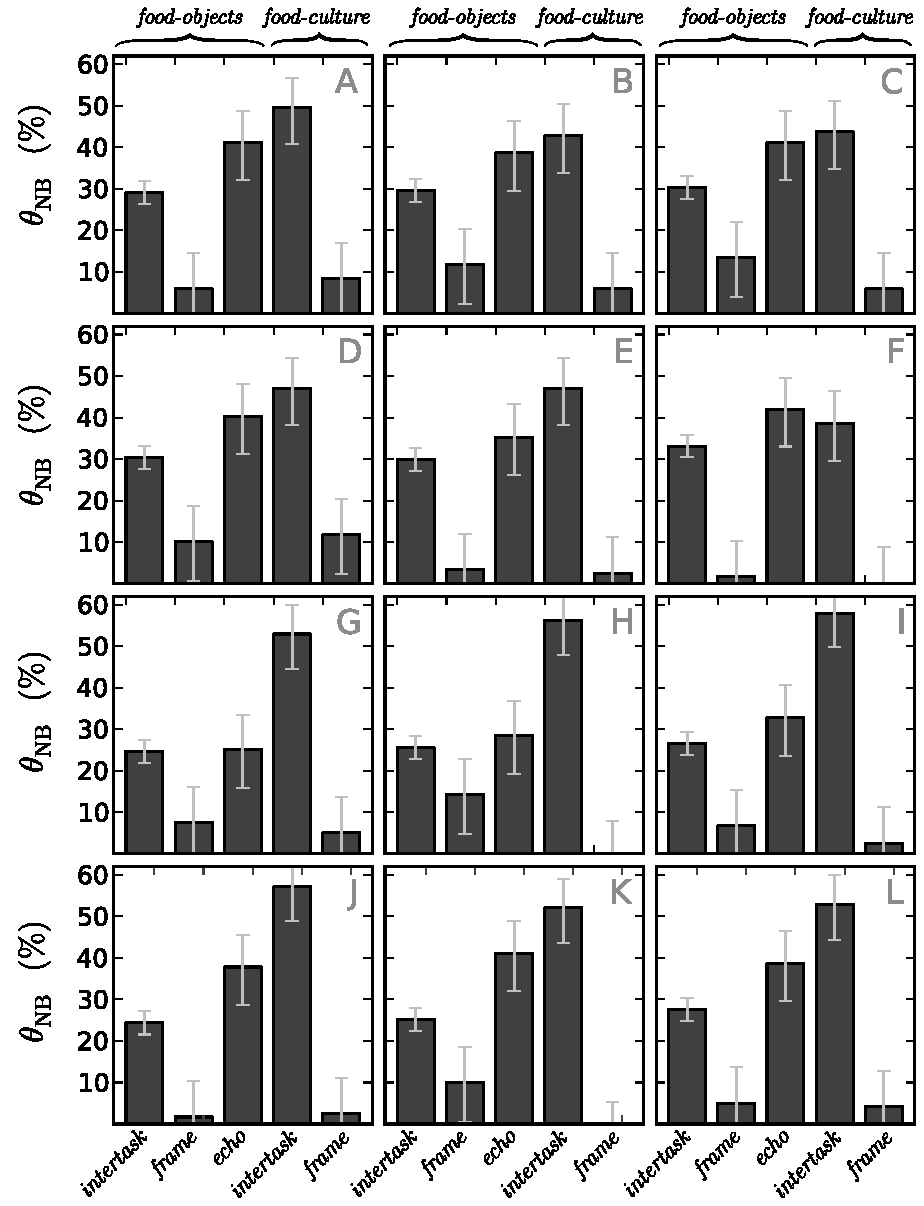
\includegraphics[scale=0.75]{figs/theta_sup.pdf}
	\label{fig:theta_sup}
	\caption{
		Figure S2: Bias induced by exposure to initial tasks and frames.
		Bias is defined to be the difference in the probability 
		distribution over workers' labels (L1-distance).  The plotted values
		give a lower bound to the L1-distance, $D_{L1}^-$, which was 
		determined from a classifier's performance in 
		distinguishing workers that had undergone different exposures.
		The bias was determined using (A-F) a na\"ive Bayes classifier, and 
		(G-L) an SVM classifier.
		In panels A through F, each plot adds an additional
		preprocessing step to those used in the previous plot; the same is 
		done for panels G through H: A,G) No 
		preprocessing; B,H) spelling correction; C,I) stopword removal; 
		D,J) lemmatization; E,K) splitting of multiple-word labels; 
		F,L) distinguishing identical labels entered in different form inputs.
	}
\end{figure}
The inequality in Eq.~\ref{l1}
asserts that a classifiers performance in predicting class membership
bounds the L1-distance between the distributions of features for the classes.
This bound is tight for the optimal classifier, and in general, the slack
depends on how the classifier is constructed.

Therefore there may exist a classifier that is 
significantly better than the one used to generate our results.  Even before
committing to a particular classifier algorithm, various decisions about
preprocessing need to be made.  For example, we chose to remove stopwords,
lemmatize, split multi-word labels, distinguish the input used to enter 
labels, and correct spelling.  All of these decisions affect the classifier
performance.  The particular classifier algorithm chosen also has a strong 
effect.

Since we did not have enough data to create a separate test set, we could not
optimize these decisions.  Doing so would lead to the inflation of the 
performance, which could then only be estimated using an independent test set.
Instead, we made principled decisions as described above.

Although we cannot optimize these decisions, it is appropriate to look at
what affect these decisions had, post-hoc.  We reproduce the plot shown in 
Fig.~\ref{fig:theta}A using different combinations of preprocessing options,
and using both the na\"ive Bayes and an SVM classifier.

Unlike the na\"ive Bayes classifier, it is necessary to tune the cost and 
gamma hyperparameters of the SVM classifier, as well as choose a kernel.
We used simulated annealing to optimize the cost and gamma settings in the
classification of $task2:food$ vs $task2:cult$.  For this reason, we expect
the bar for $task2$ in Fig.~S8G-J is likely to be an overestimate due to
overfitting on those data.

These plots show that the result shown in Fig.~\ref{fig:theta}A is 
representative, and supports the validity of the lower bounds on the 
exposures exposure effects presented in the main text, in terms of induced 
L1-distance.


\subsection*{S9: Justifications and statistical properties of classifier-based measurement of computational hysteresis}
\begin{itemize}
	\item{Relationship to L1-Distance}
	\item{Relationship to bias}
	\item{Relationship to Jenson-Shannon divergence}
	\item{Other approaches to measuring L1-distance}
	\item{Comparison to hypothesis testing using $\chi^2$}
\end{itemize}



\end{document}

